\section{Vistas archimate}

\subsubsection{Actores y Roles}

\begin{figure}[!htb]
  \begin{center}
    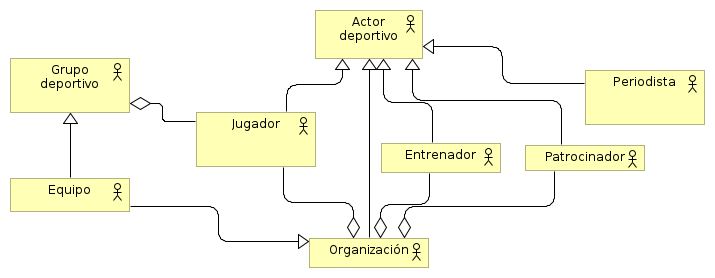
\includegraphics[width=11cm]{./imagenes/actores.png}
    \caption{Actores}
    \label{fig:Actores}
    \textbf{Fuente:}  Autores
  \end{center}
\end{figure}

\begin{table}[!htb]
	\caption{Actores}
	\label{tab:actores}
	\begin{center}
		\resizebox{11cm}{!}{
		\begin{tabular}{|p{7cm}|p{4cm}|}
			\hline
			Responsabilidades & Vistas relacionadas \\
			\hline \hline
			\begin{itemize}
				\item \textbf{Actor deportivo (Actor):} Es todo aquel actor encontrado en una red social deportiva.
				\item \textbf{Equipo (Actor):} Es un grupo deportivo conformado con el objetivo de competencia en la red social deportiva.
				\item \textbf{Patrocinador (Actor):} Prestador de servicios (monetarios, materiales o servicios deportivos tales como préstamo de espacios deportivos) que puedan ayudar o interesar a uno o más actores deportivos (jugadores y equipos) en pro de la consecución de sus objetivos.
				\item \textbf{Entrenador (Actor):} Actor deportivo cuyo objetivo es el acompañamiento y prestación de servicios de entrenamiento a los diferentes actores deportivos (jugadores/grupos deportivos/equipo).
				\item \textbf{Organización (Actor):} Organización que presta servicios deportivos a los demás actores en la red social deportiva.
				\item \textbf{Jugador (Actor):} Actor deportivo individual (persona individual) practicante de uno o varios deportes.
				\item \textbf{Periodista (Actor):} Actor cuyo objetivo es el de proporcionar información acerca de los diferentes acontecimientos ocurridos en el deporte alrededor del mundo.
				\item \textbf{Grupo deportivo (Actor):} Es un grupo deportivo conformado con el objetivo recreacional de practicar uno o varios deportes.
			\end{itemize} 
			&
			\begin{itemize}
				\item N/A
			\end{itemize} 
			\\
			\hline
		\end{tabular}
		} \\
		\textbf{Fuente}: Autores
	\end{center}
\end{table}

\begin{figure}[!htb]
  \begin{center}
    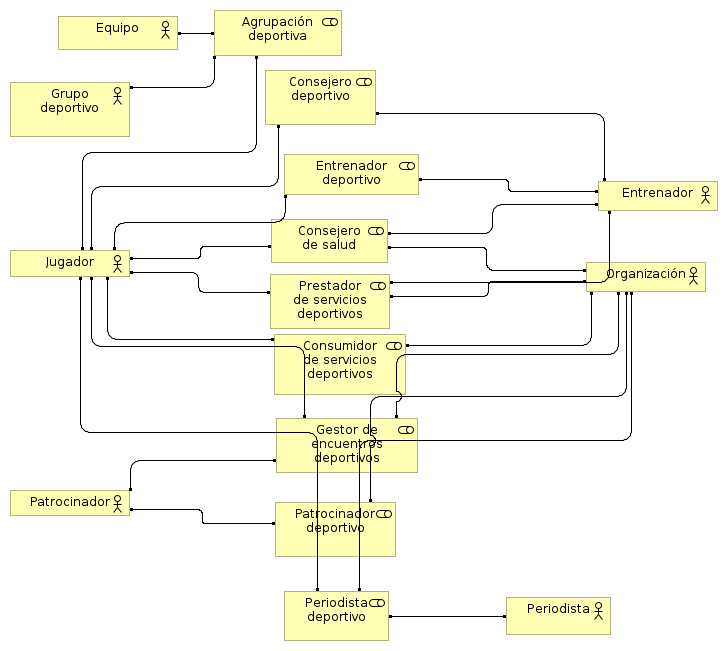
\includegraphics[width=11cm]{./imagenes/roles.png}
    \caption{Roles}
    \label{fig:Roles}
    \textbf{Fuente:}  Autores
  \end{center}
\end{figure}

\begin{table}[!htb]
	\caption{Actores}
	\label{tab:actores}
	\begin{center}
		\resizebox{11cm}{!}{
		\begin{tabular}{|p{7cm}|p{4cm}|}
			\hline
			Responsabilidades & Vistas relacionadas \\
			\hline \hline
			\begin{itemize}
				\item \textbf{Agrupación deportiva (Rol):} Grupo deportivo o equipo deportivo que se reunen a practicar un deporte.
				\item \textbf{Consejero deportivo (Rol):} Jugador/entrenador dador de consejos deportivos.
				\item \textbf{Entrenador deportivo (Rol):} Quien cumple la función de entrenar.
				\item \textbf{Consejero de salud (Rol):} Jugador/entrenador/organización encargados de dar consejos de salud dentro de la red social deportiva.
				\item \textbf{Prestador de servicios deportivos (Rol):} Actor deportivo que ofrece sus servicios a los demás actores en la red social.
				\item \textbf{Consumidor de servicios deportivos (Rol):} Actor deportivo que consume el servicio otorgado por un prestador de servicios deportivos.
				\item \textbf{Gestor de encuentros deportivos (Rol):} Gestor de un encuentro deportivo.
				\item \textbf{Patrocinador deportivo (Rol):} Actor deportivo que apoya a un jugador/equipo/evento en la consecución de sus metas otorgandole dinero, materiales o servicios deportivos.
				\item \textbf{Periodista deportivo (Rol):} Actor que publica información deportiva de diversa índole alrededor del mundo.
			\end{itemize} 
			&
			\begin{itemize}
				\item Bussiness process (Entrenamiento deportivo, estadísticas deportivas, organización de eventos deportivos, formación de grupos deportivos, patrocinios deportivos), Business function (Patrocinio deportivo, Entrenamiento deportivo, Estadísticas deportivas, Formación de grupos deportivos, Organización de eventos deportivos)
				\item Bussiness process (Entrenamiento deportivo), Business function (Entrenamiento deportivo)
				\item Bussiness process (Entrenamiento deportivo, estadísticas deportivas, formación de grupos deportivos, patrocinios deportivos), Business function (Patrocinio deportivo, Entrenamiento deportivo, Estadísticas deportivas, Formación de grupos deportivos)
				\item N/A
				\item N/A
				\item N/A
				\item Bussiness process (Patrocinio deportivo, Organización evento deportivo), Business function (Organización eventos deportivos, Patrocinios deportivos)
				\item Bussiness process (Estadísticas deportivas), Business function (Patrocinio deportivo, Estadísticas deportivas, Organizador de eventos deportivos)
				\item N/A
			\end{itemize} 
			\\
			\hline
		\end{tabular}
		} \\
		\textbf{Fuente}: Autores
	\end{center}
\end{table}

\subsubsection{Introductory viewpoint}

\begin{figure}[!htb]
  \begin{center}
    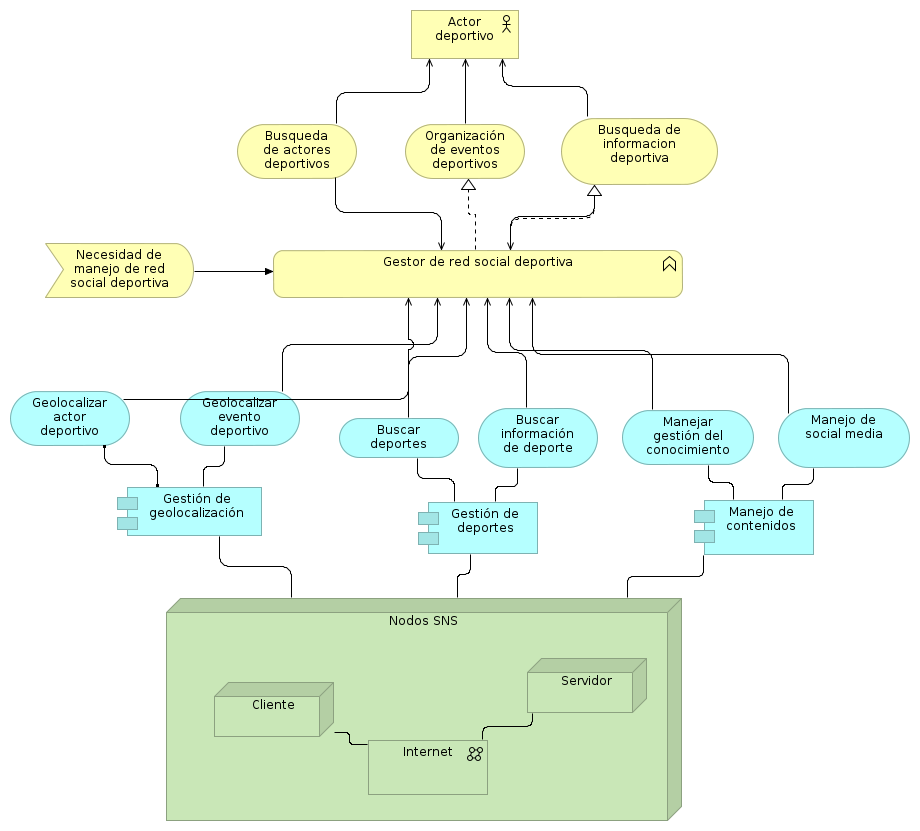
\includegraphics[width=11cm]{./imagenes/introductory.png}
    \caption{Punto de vista introductorio}
    \label{fig:introductory}
    \textbf{Fuente:}  Autores
  \end{center}
\end{figure}

\begin{table}[!htb]
	\caption{Punto de vista introductorio}
	\label{tab:introductory}
	\begin{center}
		\resizebox{11cm}{!}{
		\begin{tabular}{|p{7cm}|p{4cm}|}
			\hline
			Responsabilidades & Vistas relacionadas \\
			\hline \hline
			
			\begin{itemize}
				\item \textbf{Búsqueda de información deportiva (Servicio de negocio):} Usado para buscar información relacioana con el deporte: Reglas, consejos deportivos, entre otros.
				\item \textbf{Organización de eventos deportivos (Servicio de negocio):} Servicio por medio del cual todos los actores participantes componen un evento deportivo (ya sea un torneo, una clínica deportiva, un entrenamiento o partido(s) aislado(s)).
				\item \textbf{Buscar deportes (Servicio de aplicación):} Permite la búsqueda de los deportes existentes en la red social deportiva, teniendo la posibilidad de elegir ciertos criterios de búsqueda especificados en los requerimientos.
				\item \textbf{Buscar información de deporte (Servicio de aplicación):} Permite el acceso y búsqueda sobre una base de conocimiento acerca del deporte buscado previamente.
				\item \textbf{Geolocalizar evento deportivo (Servicio de aplicación):} Deja al usuario del SNS localizar un evento por medio de las funcionalidades de geolocalización prestadas por el dispositivo utilizado y utilizadas por el mismo SNS.
				\item \textbf{Geolocalizar actor deportivo (Servicio de aplicación):} Deja al usuario del SNS localizar un actor deportivo por medio de las funcionalidades de geolocalización prestadas por el dispositivo utilizado y utilizadas por el mismo SNS.
				\item \textbf{Manejar gestión del conocimiento (Servicio de aplicación):} Servicio que administra las funcionalidades proporcionadas en el acceso a la base de conocimiento.
				\item \textbf{Manejo de social media (Servicio de aplicación):} Servicio que permite manejar funcionalidades social media (publicación de información, comunicación por chats, comentarios a publicaciones públicas en un perfíl propio del actor deportivo).
				\item \textbf{Gestión de geolocalización (Componente de aplicación):} Componente utilizado por otros para la ubicación de eventos y grupos deportivos/jugadores en el SNS.
				\item \textbf{Gestión de deportes (Componente de aplicación):} Deja al usuario administrador del SNS, así como a otros servicios de aplicación, crear, modificar o recuperar la información de un deporte en específico soportado por el SNS.
				\item \textbf{Manejo de contenidos (Componente de aplicación):} Componente del SNS para la administración de los contenidos, referiendose a la base de conocimientos proporcionada para cada deporte soportado por la red social.
				\item \textbf{Necesidad de manejo de red social deportiva (Evento):} Lanzador de las funciones de administrador de red social deportiva.
				\item \textbf{Actor deportivo (Actor):} Es todo aquel actor encontrado en una red social deportiva.
				\item \textbf{Busqueda de actores deportivos (Servicio de negocio):} Ofrece la búsqueda de cualquier actor participante en la red social deportiva.
			\end{itemize} 
			&
			\begin{itemize}
				\item Por capas, introductorio
				\item Por capas, introductorio
				\item Por capas, introductorio
				\item Por capas, introductorio
				\item Por capas, introductorio
				\item Por capas, introductorio
				\item Por capas, introductorio
				\item Por capas, introductorio, Bussiness process - Application usage - (Formación de grupos deportivos)
				\item Por capas, introductorio, Application usage - (Estadísticas deportivas, Organización eventos deportivos)
				\item Por capas, introductorio
				\item Por capas, introductorio, Application usage - (Entrenamiento deportivo, Estadísticas deportivas)
				\item Por capas, introductorio
				\item Por capas, introductorio
				\item N/A
			\end{itemize} 
			\\
			\hline
		\end{tabular}
		} \\
		\textbf{Fuente}: Autores
	\end{center}
\end{table}

\subsubsection{Layered viewpoint}

\begin{figure}[!htb]
  \begin{center}
    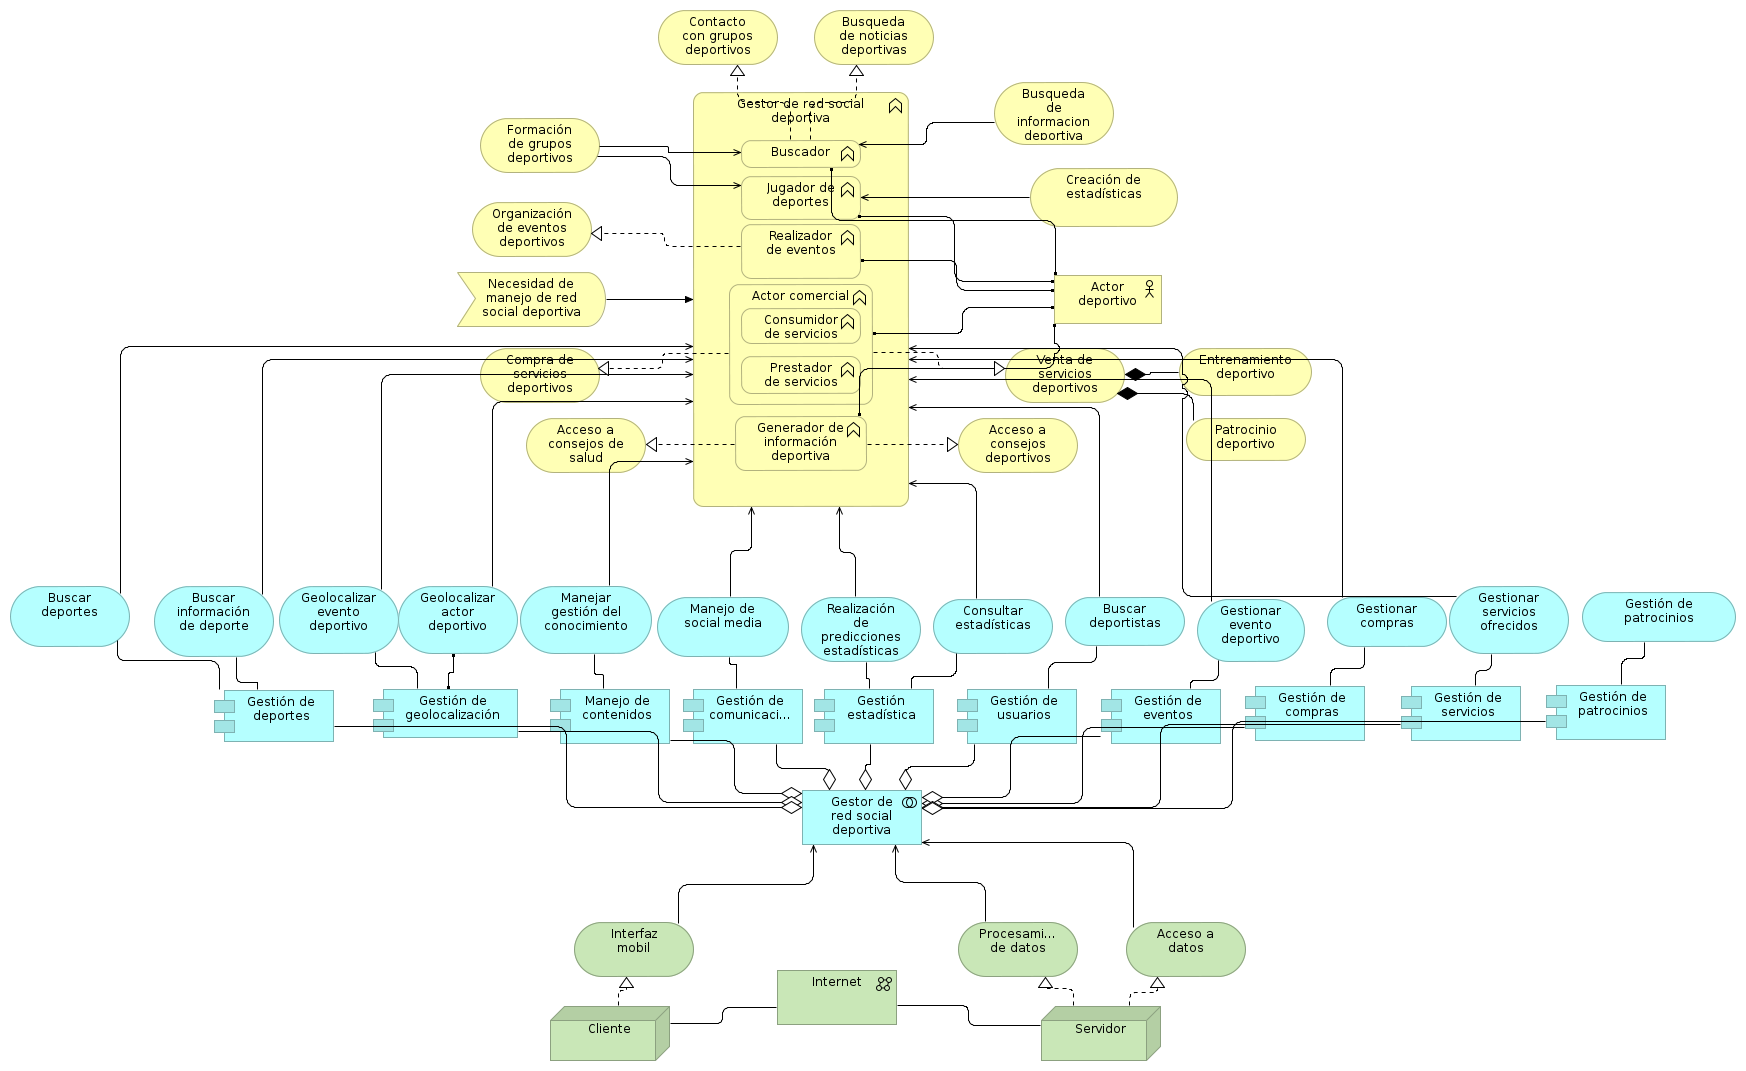
\includegraphics[width=11cm]{./imagenes/generallayered.png}
    \caption{Punto de Vista General por Capas}
    \label{fig:general_layered}
    \textbf{Fuente:}  Autores
  \end{center}
\end{figure}

\subsection{Business Functions Viewpoints}

\subsubsection{Patrocinios Deportivos}

\begin{figure}[!htb]
  \begin{center}
    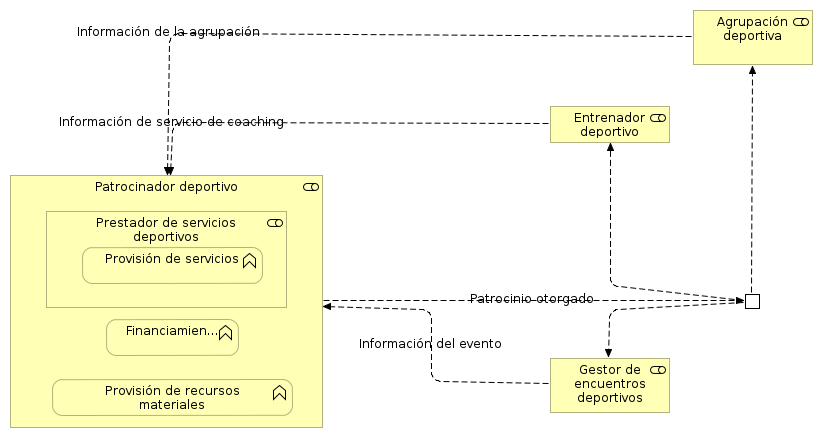
\includegraphics[width=11cm]{./imagenes/business_functions/patrociniosdeportivos.png}
    \caption{Patrocinios Deportivos}
    \label{fig:patrocinios_deportivos}
    \textbf{Fuente:}  Autores
  \end{center}
\end{figure}

\begin{table}[!htb]
	\caption{Business function - Patrocinio Deportivo}
	\label{tab:BF_PatrocinioDeportivo}
	\begin{center}
		\resizebox{11cm}{!}{
		\begin{tabular}{|p{7cm}|p{4cm}|}
			\hline
			Responsabilidades & Vistas relacionadas \\
			\hline \hline
			Función encargada de facilitar el acceso a la información relacionada a grupos deportivos existentes.
			\begin{itemize}
				\item \textbf{Patrocinador deportivo (Rol):} Actor deportivo que apoya a un jugador/equipo/evento en la consecución de sus metas otorgandole dinero, materiales o servicios deportivos.
				\item \textbf{Prestador de servicios deportivos (Rol):} Actor deportivo que ofrece sus servicios a los demás actores en la red social.
				\item \textbf{Agrupación deportiva (Rol):} Grupo deportivo o equipo deportivo que se reunen a practicar un deporte.
				\item \textbf{Entrenador deportivo (Rol):} Quien cumple la función de entrenar.
				\item \textbf{Gestor de encuentros deportivos (Rol):} Gestor de un encuentro deportivo.
				\item \textbf{Financiamiento (Función):} Función desarrollada por un patrocinador deportivo para patrocinar a otros entes en la red social.
				\item \textbf{Provisión de recursos materiales (Función):} Función cumplida por un patrocinador deportivo, dando a las agrupaciones que patrocina recursos materiales.
				\item \textbf{Provisión de servicios (Función):} Función cumplida por un patrocinador deportivo, dando a las agrupaciones que patrocina servicios que él ofrezca.
			\end{itemize} 
			&
			\begin{itemize}
				\item Rol - actor, Bussiness process (Estadísticas deportivas), Business function (Estadísticas deportivas, Organizador de eventos deportivos)
				\item Rol - actor
				\item Rol - actor, Bussiness process (Entrenamiento deportivo, estadísticas deportivas, organización de eventos deportivos, formación de grupos deportivos, patrocinios deportivos), Business function (Entrenamiento deportivo, Estadísticas deportivas, Formación de grupos deportivos, Organización de eventos deportivos)
				\item Rol - actor, Bussiness process (Entrenamiento deportivo, estadísticas deportivas, formación de grupos deportivos, patrocinios deportivos), Business function (Entrenamiento deportivo, Estadísticas deportivas, Formación de grupos deportivos)
				\item Rol - actor, Bussiness process (Patrocinio deportivo, Organización evento deportivo), Business function (Organización eventos deportivos)
				\item Application usage (Organización de eventos deportivos), Business function (Organización de eventos deportivos), Business process (Organización de eventos deportivos)
				\item Application usage (Organización de eventos deportivos), Business function (Organización de eventos deportivos), Business process (Organización de eventos deportivos)
				\item Application usage (Organización de eventos deportivos), Business function (Organización de eventos deportivos), Business process (Organización de eventos deportivos)
			\end{itemize} 
			\\
			\hline
		\end{tabular}
		} \\
		\textbf{Fuente}: Autores
	\end{center}
\end{table}

\subsubsection{Organización de Eventos Deportivos}

\begin{figure}[!htb]
  \begin{center}
    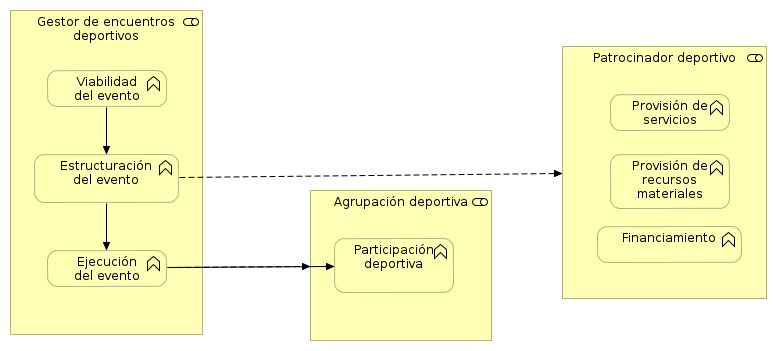
\includegraphics[width=11cm]{./imagenes/business_functions/organizacioneventosdeportivos.png}
    \caption{Organización de Eventos Deportivos}
    \label{fig:organizacion_eventos_deportivos}
    \textbf{Fuente:}  Autores
  \end{center}
\end{figure}

\begin{table}[!htb]
	\caption{Business function - Organización de eventos deportivos}
	\label{tab:BF_OrganizacionEventosDeportivos}
	\begin{center}
		\resizebox{11cm}{!}{
		\begin{tabular}{|p{7cm}|p{4cm}|}
			\hline
			Responsabilidades & Vistas relacionadas \\
			\hline \hline
			\begin{itemize}
				\item \textbf{Gestor de encuentros deportivos (Rol):} Gestor de un encuentro deportivo.
				\item \textbf{Agrupación deportiva (Rol):} Grupo deportivo o equipo deportivo que se reunen a practicar un deporte
				\item \textbf{Patrocinador deportivo (Rol):} Actor deportivo que apoya a un jugador/equipo/evento en la consecución de sus metas otorgandole dinero, materiales o servicios deportivos
				\item \textbf{Verificación viabilidad del evento (Función):} Función que realiza un actor para verificar que un evento es viable o no de hacer
				\item \textbf{Estructuración del evento (Función):} Función desarrollada por los entes que estructuran un evento deportivo, antes de su ejecución real
				\item \textbf{Ejecución del evento (Función):} Función realizada por los entes involucrados en la ejecución de la planeación de un evento deportivo
				\item \textbf{Participación deportiva (Función):} Función que desempeñan aquellas agrupaciones deportivas que fueron invitadas o aceptadas en un evento deportivo. Esta se refiere a toda actividad que ellos deban hacer
				\item \textbf{Provisión de servicios (Función):} Función cumplida por un patrocinador deportivo, dando a las agrupaciones que patrocina servicios que él ofrezca
				\item \textbf{Provisión de recursos materiales (Función):} Función cumplida por un patrocinador deportivo, dando a las agrupaciones que patrocina recursos materiales
				\item \textbf{Financiamiento (Función):} Función desarrollada por un patrocinador deportivo para patrocinar a otros entes en la red social
			\end{itemize} 
			&
			\begin{itemize}
				\item Rol - actor, Bussiness process (Patrocinio deportivo, Organización evento deportivo), Business function (Patrocinios deportivos)
				\item Rol - actor, Bussiness process (Entrenamiento deportivo, estadísticas deportivas, organización de eventos deportivos, formación de grupos deportivos, patrocinios deportivos), Business function (Patrocinio deportivo, Entrenamiento deportivo, Estadísticas deportivas, Formación de grupos deportivos)
				\item Rol - actor, Bussiness process (Estadísticas deportivas), Business function (Patrocinio deportivo, Estadísticas deportivas)
				\item N/A
				\item N/A
				\item N/A
				\item N/A
				\item Application usage (Organización de eventos deportivos), Business function (Patrocinios deportivos), Business process (Organización de eventos deportivos)
				\item Application usage (Organización de eventos deportivos), Business function (Patrocinios deportivos), Business process (Organización de eventos deportivos)
				\item Application usage (Organización de eventos deportivos), Business function (Patrocinios deportivos), Business process (Organización de eventos deportivos)
			\end{itemize} 
			\\
			\hline
		\end{tabular}
		} \\
		\textbf{Fuente}: Autores
	\end{center}
\end{table}

\subsubsection{Formación de Grupos Deportivos}

\begin{figure}[!htb]
  \begin{center}
    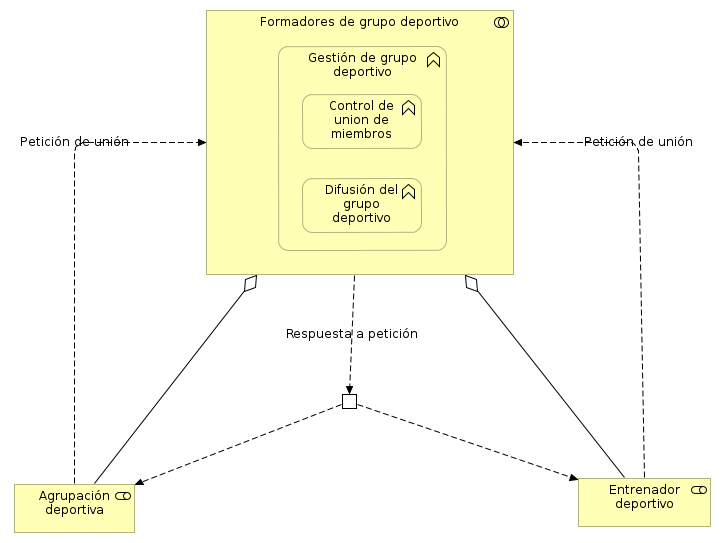
\includegraphics[width=11cm]{./imagenes/business_functions/formaciongruposdeportivos.png}
    \caption{Formación de Grupos Deportivos}
    \label{fig:formacion_grupos_deportivos}
    \textbf{Fuente:}  Autores
  \end{center}
\end{figure}

\begin{table}[!htb]
	\caption{Business function - Formación de Grupos Deportivos}
	\label{tab:BF_FormacionGruposDeportivos}
	\begin{center}
		\resizebox{11cm}{!}{
		\begin{tabular}{|p{7cm}|p{4cm}|}
			\hline
			Responsabilidades & Vistas relacionadas \\
			\hline \hline
			\begin{itemize}
				\item \textbf{Formadores de grupo deportivo (Colaboración):} Colaboración conformada por los roles que trabajan en la dinámica de un grupo deportivo a traves del tiempo
				\item \textbf{Agrupación deportiva (Rol):} Grupo deportivo o equipo deportivo que se reunen a practicar un deporte
				\item \textbf{Entrenador deportivo (Rol):} Quien cumple la función de entrenar
				\item \textbf{Gestión de grupo deportivo (Función):} Función que desarrolla el ente encargado de gestionar aspectos internos o externos relacionados con el grupo deportivo al que gestiona
				\item \textbf{Difusión del grupo deportivo (Función):} Función realizada por el ente que difunde el grupo deportivo en los diferentes canales de la red social
				\item \textbf{Control de unión de miembros(Función):} Función asignada a quien controla la unión de gente nueva a un grupo deportivo
				\item \textbf{Difusión de información deportiva (Función):} 
			\end{itemize} 
			&
			\begin{itemize}
				\item Bussiness process (Formación de grupos deportivos)
				\item Rol - actor, Bussiness process (Entrenamiento deportivo, estadísticas deportivas, organización de eventos deportivos, formación de grupos deportivos, patrocinios deportivos), Business function (Patrocinio deportivo, Entrenamiento deportivo, Estadísticas deportivas, Organización de eventos deportivos)
				\item Rol - actor, Bussiness process (Entrenamiento deportivo, estadísticas deportivas, formación de grupos deportivos, patrocinios deportivos), Business function (Patrocinio deportivo, Entrenamiento deportivo, Estadísticas deportivas)
				\item N/A
				\item N/A
				\item N/A
				\item 
			\end{itemize} 
			\\
			\hline
		\end{tabular}
		} \\
		\textbf{Fuente}: Autores
	\end{center}
\end{table}

\subsubsection{Estadísticas Deportivas}

\begin{figure}[!htb]
  \begin{center}
    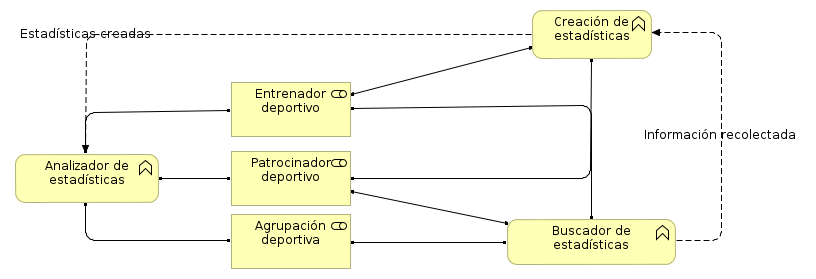
\includegraphics[width=11cm]{./imagenes/business_functions/estadisticasdeportivas.png}
    \caption{Estadísticas Deportivas}
    \label{fig:estadisticas_deportivas}
    \textbf{Fuente:}  Autores
  \end{center}
\end{figure}

\begin{table}[!htb]
	\caption{Business function - Estadísticas Deportivas}
	\label{tab:BF_EstadisticasDeportivas}
	\begin{center}
		\resizebox{11cm}{!}{
		\begin{tabular}{|p{7cm}|p{4cm}|}
			\hline
			Responsabilidades & Vistas relacionadas \\
			\hline \hline
			\begin{itemize}
				\item \textbf{Patrocinador deportivo (Rol):} Actor deportivo que apoya a un jugador/equipo/evento en la consecución de sus metas otorgandole dinero, materiales o servicios deportivos
				\item \textbf{Agrupación deportiva (Rol):} Grupo deportivo o equipo deportivo que se reunen a practicar un deporte
				\item \textbf{Entrenador deportivo (Rol):} Quien cumple la función de entrenar
				\item \textbf{Buscador de estadísticas (Función):} Función realizada por quien se dedica a buscar estadísticas deportivas
				\item \textbf{Creación de estadísticas (Función):} Función realizada por el ente creador de estadísticas
				\item \textbf{Analizador de estadísticas (Función):} Función asignada a quien analiza estadísticas deportivas
			\end{itemize} 
			&
			\begin{itemize}
				\item Rol - actor, Bussiness process (Estadísticas deportivas), Business function (Patrocinio deportivo, Organizador de eventos deportivos)
				\item Rol - actor, Bussiness process (Entrenamiento deportivo, estadísticas deportivas, organización de eventos deportivos, formación de grupos deportivos, patrocinios deportivos), Business function (Patrocinio deportivo, Entrenamiento deportivo, Estadísticas deportivas, Organización de eventos deportivos)
				\item Rol - actor, Bussiness process (Entrenamiento deportivo, estadísticas deportivas, formación de grupos deportivos, patrocinios deportivos), Business function (Patrocinio deportivo, Entrenamiento deportivo, Estadísticas deportivas)
				\item N/A
				\item N/A
				\item N/A
			\end{itemize} 
			\\
			\hline
		\end{tabular}
		} \\
		\textbf{Fuente}: Autores
	\end{center}
\end{table}

\subsubsection{Entrenamiento Deportivo}

\begin{figure}[!htb]
  \begin{center}
    \includegraphics[width=11cm]{./imagenes/business_functions/entrenamientodeportivo.png}
    \caption{Entrenamiento Deportivo}
    \label{fig:entrenamiento_deportivo}
    \textbf{Fuente:}  Autores
  \end{center}
\end{figure}

\begin{table}[!htb]
	\caption{Business function - Entrenamiento Deportivo}
	\label{tab:BF_EntrenamientoDeportivo}
	\begin{center}
		\resizebox{11cm}{!}{
		\begin{tabular}{|p{7cm}|p{4cm}|}
			\hline
			Responsabilidades & Vistas relacionadas \\
			\hline \hline
			\begin{itemize}
				\item \textbf{Consejero deportivo (Rol):} Jugador/entrenador dador de consejos deportivos
				\item \textbf{Agrupación deportiva (Rol):} Grupo deportivo o equipo deportivo que se reunen a practicar un deporte
				\item \textbf{Entrenador deportivo (Rol):} Quien cumple la función de entrenar
				\item \textbf{Consejero deportivo (Función):} Ésta es realizada por la persona quien ayuda paso a paso a los deportistas en las agrupaciones deportivas a realizarse en sus habilidades humanas y deportivas
				\item \textbf{Entrenador (Función):} Función cumplida por el ente que entrena a los miembros de una agrupación deportiva
				\item \textbf{Creador de ejercicios (Función):} Función realizada por el ente que crea ejercicios que serán realizados por los miembros de una agrupación deportiva en un entrenamiento
				\item \textbf{Evaluador de grupo deportivo (Función):} Función realizada por el ente que vigila el rendimiento de las personas que pertenecen a un grupo deportivo
				\item \textbf{Entrenar (Función):} Función desempeñada por los miembros de una agrupación deportiva que siguen los ejercicios asignados por aquel que tenga la función de ser entrenador, así como ser coevaluador
				\item \textbf{Practicante de ejercicios (Función):} Función desempeñada por los miembros de una agrupación deportiva, realizar los ejercicios asignados por un entrenador
				\item \textbf{Coevaluador (Función):} Función realizada por deportistas de la misma agrupación deportiva quienes juzgan el trabajo de los compañeros
			\end{itemize} 
			&
			\begin{itemize}
				\item Rol - actor, Bussiness process (Entrenamiento deportivo)
				\item Rol - actor, Bussiness process (Entrenamiento deportivo, estadísticas deportivas, organización de eventos deportivos, formación de grupos deportivos, patrocinios deportivos), Business function (Patrocinio deportivo, Estadísticas Deportivas, Formación de Grupos Deportivos, Organización de eventos deportivos)
				\item Rol - actor, Bussiness process (Entrenamiento deportivo, estadísticas deportivas, formación de grupos deportivos, patrocinios deportivos), Business function (Patrocinio deportivo, Formación de Grupos Deportivos, Estadísticas Deportivas)
				\item N/A
				\item N/A
				\item N/A
				\item N/A
				\item N/A
				\item N/A
				\item N/A
			\end{itemize} 
			\\
			\hline
		\end{tabular}
		} \\
		\textbf{Fuente}: Autores
	\end{center}
\end{table}

\subsubsection{Buscador Deportivo}

\begin{figure}[!htb]
  \begin{center}
    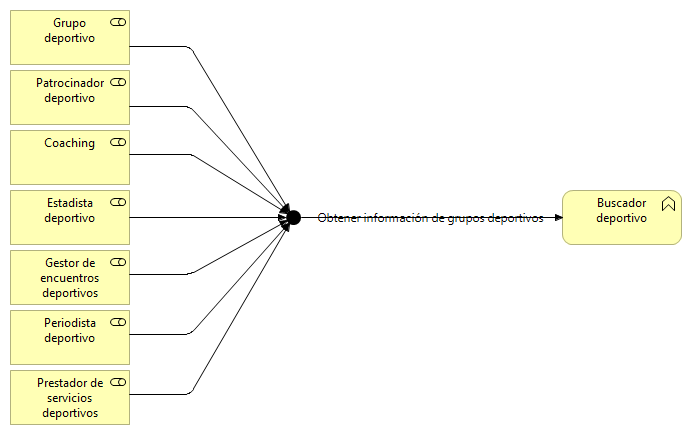
\includegraphics[width=11cm]{./imagenes/business_functions/buscadordeportivo.png}
    \caption{Buscador deportivo}
    \label{fig:BF_BuscadorDeportivo}
    \textbf{Fuente:}  Autores
  \end{center}
\end{figure}

\begin{table}[!htb]
	\caption{Descripción Buscador Deportivo}
	\label{tab:BF_BuscadorDeportivo}
	\begin{center}
		\resizebox{11cm}{!}{
		\begin{tabular}{|p{7cm}|p{4cm}|}
			\hline
			Responsabilidades & Vistas relacionadas \\
			\hline \hline
			Función encargada de facilitar el acceso a la información relacionada a grupos deportivos existentes.
			\begin{itemize}
				\item \textbf{Grupo deportivo (Rol):} Asociación de uno o más deportistas que practican por lo menos un deporte en común
				\item \textbf{SNS Deportivo (Rol):} Aplicación o facilitador para la búsqueda y contacto de grupos deportivos
				\item \textbf{Patrocinador deportivo (Rol):} Persona o entidad que brinda patrocinios (Equipamiento, dinero, bienes, servicios, etc.) a deportistas, grupos deportivos o eventos
				\item \textbf{Buscador deportivo (Función):} Función asociada al rol de SNS Deportivo que se ejecuta para buscar un grupo deportivo según un criterio dado.
			\end{itemize} 
			&
			\begin{itemize}
				\item N/A
			\end{itemize} 
			\\
			\hline
		\end{tabular}
		} \\
		\textbf{Fuente}: Autores
	\end{center}
\end{table}

\subsubsection{Consejos}

\begin{figure}[!htb]
  \begin{center}
    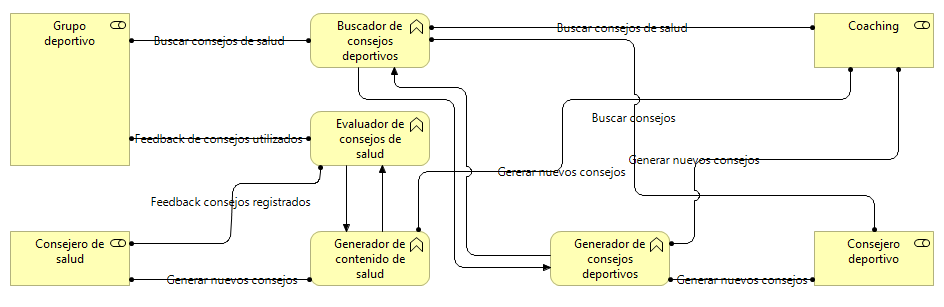
\includegraphics[width=11cm]{./imagenes/business_functions/Consejos.png}
    \caption{Consejos}
    \label{fig:BF_Consejos}
    \textbf{Fuente:}  Autores
  \end{center}
\end{figure}

\begin{table}[!htb]
	\caption{Descripción Consejos}
	\label{tab:BF_Consejos}
	\begin{center}
		\resizebox{11cm}{!}{
		\begin{tabular}{|p{7cm}|p{4cm}|}
			\hline
			Responsabilidades & Vistas relacionadas \\
			\hline \hline
			Administra la generación y consultas de consejos orientados a las temáticas de salud o contenidos deportivos.
			\begin{itemize}
				\item \textbf{Grupo deportivo (Rol):} Asociación de uno o más deportistas que practican por lo menos un deporte en común
				\item \textbf{Consejero de salud (Rol):} Experto en temas de salud relacionados con la práctica de un deporte, acondicionamiento físico, etc.
				\item \textbf{Coaching (Rol):} Experto en temas relacionados con la práctica de un deporte.
				\item \textbf{Consejero deportivo (Rol):} Experto en temas relacionados a la práctica de uno o varios deportes.
				\item \textbf{SNS Deportivo (Rol):} Aplicación o facilitador para la búsqueda y retroalimentación de consejos deportivos.
				\item \textbf{Buscador de consejos deportivos (Función):} Función asociada a los roles de Coaching y Grupo deportivo que les permite el acceso a la base de conocimientos asociados a consejos deportivos.
				\item \textbf{Evaluador de consejos de salud (Función):} Función asociada a los roles de Coaching, Grupo deportivo y consejero de salud que les permite dar una retroalimentación acerca de que tan útil le resulta un consejo de salud existente.
				\item \textbf{Generador de contenido de salud (Función):} Función asociada a los roles de Coaching y consejero de salud que les permite crear un consejo sobre algún tema de interés para la comunidad deportiva que estérelacionado con la salud.
				\item \textbf{Generador de consejos deportivos (Función):} Función asociada al rol de Coaching que le permite crear un consejo sobre algún tema de interés para la comunidad deportiva que estérelacionado con la práctica de algún deporte.
			\end{itemize} 
			&
			\begin{itemize}
				\item N/A
			\end{itemize} 
			\\
			\hline
		\end{tabular}
		} \\
		\textbf{Fuente}: Autores
	\end{center}
\end{table}

\subsubsection{Periodismo}

\begin{figure}[!htb]
  \begin{center}
    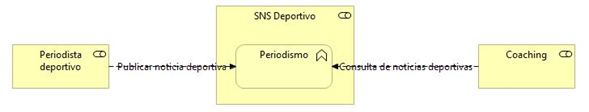
\includegraphics[width=11cm]{./imagenes/business_functions/Periodismo.png}
    \caption{Periodismo}
    \label{fig:BF_Periodismo}
    \textbf{Fuente:}  Autores
  \end{center}
\end{figure}

\begin{table}[!htb]
	\caption{Descripción Periodismo}
	\label{tab:BF_Periodismo}
	\begin{center}
		\resizebox{11cm}{!}{
		\begin{tabular}{|p{7cm}|p{4cm}|}
			\hline
			Responsabilidades & Vistas relacionadas \\
			\hline \hline
			Función encargada de administrar la generación y consulta de noticias deportivas.
			\begin{itemize}
				\item \textbf{Periodista deportivo (Rol):} Persona o Asociación que, luego de un trabajo de investigación y edición, publica una noticia relacionada a algún tema deportivo.
				\item \textbf{Coaching (Rol):} Experto en temas relacionados con la práctica de un deporte.
				\item \textbf{SNS Deportivo (Rol):} Aplicación o facilitador para la búsqueda y publicación de noticias deportivas.
				\item \textbf{Periodismo (Función):} Función que le permite a un periodista deportivo publicar una noticia deportiva y a un coach consultar las noticias publicadas.
			\end{itemize} 
			&
			\begin{itemize}
				\item N/A
			\end{itemize} 
			\\
			\hline
		\end{tabular}
		} \\
		\textbf{Fuente}: Autores
	\end{center}
\end{table}

\subsubsection{Servicios}

\begin{figure}[!htb]
  \begin{center}
    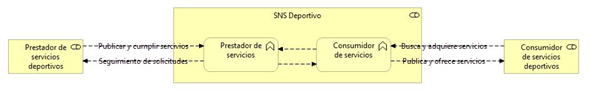
\includegraphics[width=11cm]{./imagenes/business_functions/Servicios.png}
    \caption{Servicios}
    \label{fig:BF_Servicios}
    \textbf{Fuente:}  Autores
  \end{center}
\end{figure}

\begin{table}[!htb]
	\caption{Descripción Servicios}
	\label{tab:BF_Servicios}
	\begin{center}
		\resizebox{11cm}{!}{
		\begin{tabular}{|p{7cm}|p{4cm}|}
			\hline
			Responsabilidades & Vistas relacionadas \\
			\hline \hline
			Administra el consumo y oferta de servicios deportivos a los interesados.
			\begin{itemize}
				\item \textbf{Prestador de servicios deportivos (Rol):} Persona o Asociación que ofrece un bien o servicio (Gratuito o de pago).
				\item \textbf{Consumidor  de servicios deportivos (Rol):} Persona o Asociación que adquiere (consume) un servicio que es ofrecido por un Prestador de servicios.
				\item \textbf{SNS Deportivo:} Aplicación o facilitador para la búsqueda y contacto entre el prestador y consumidor de servicios.
				\item \textbf{Prestador de servicios (Función):} Función asociada al rol de prestador de servicios deportivos que facilita la gestión y publicación de los servicios que se ofrecen a los interesados.
				\item \textbf{Consumidor de servicios (Función):} Función asociada al rol de consumidor de servicios deportivos que facilita la gestión y búsqueda de los servicios que se tienen contratados o se desean contratar.
			\end{itemize} 
			&
			\begin{itemize}
				\item Coaching
				\item Consejero deportivo
				\item Consejero de salud
				\item Grupo deportivo
			\end{itemize} 
			\\
			\hline
		\end{tabular}
		} \\
		\textbf{Fuente}: Autores
	\end{center}
\end{table}

\subsection{Business Process Viewpoints}

\subsubsection{Patrocinios Deportivos}

\begin{figure}[!htb]
  \begin{center}
    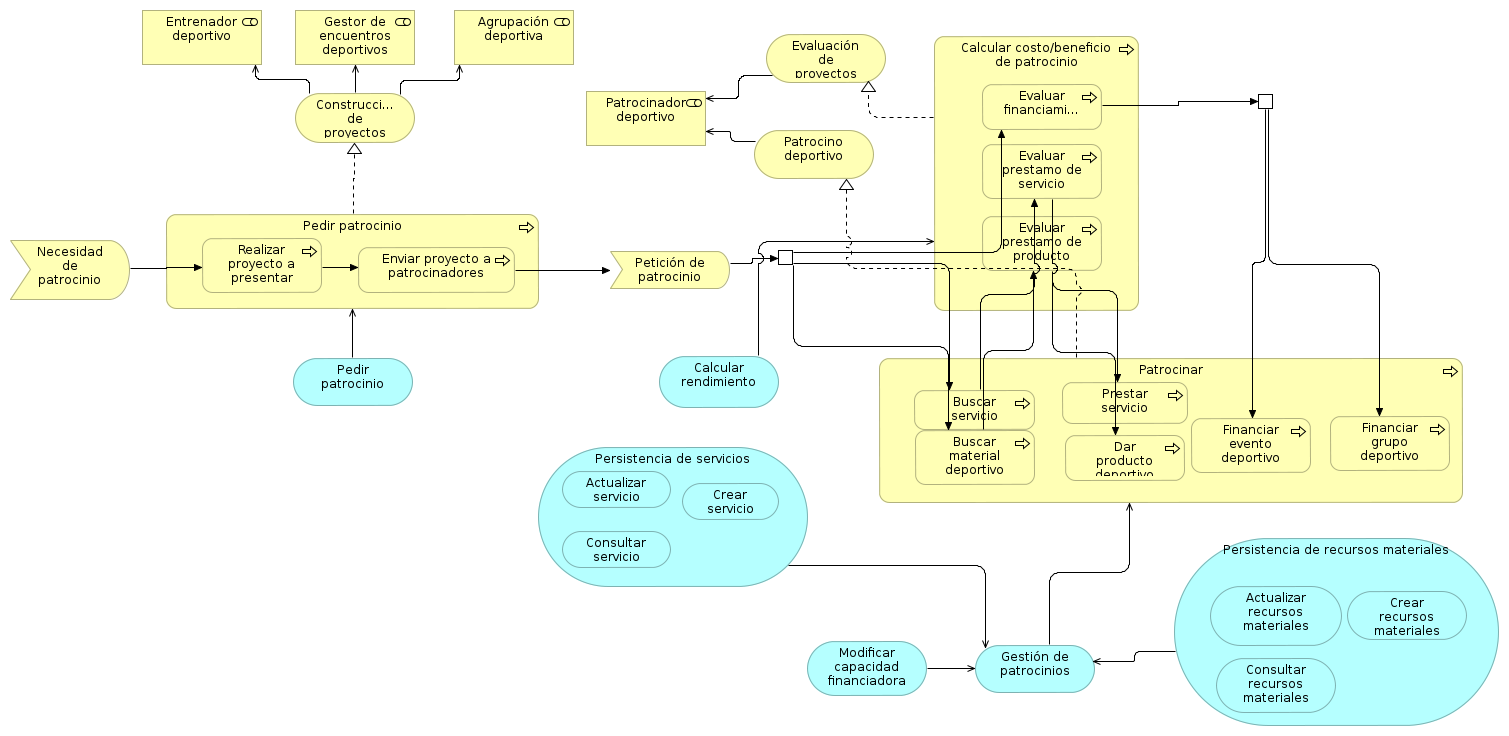
\includegraphics[width=11cm]{./imagenes/business_process/patrociniosdeportivos.png}
    \caption{Buscador deportivo}
    \label{fig:BF_BuscadorDeportivo}
    \textbf{Fuente:}  Autores
  \end{center}
\end{figure}

\begin{table}[!htb]
	\caption{Patrocinios Deportivos}
	\label{tab:BP_PatrociniosDeportivos}
	\begin{center}
		\resizebox{11cm}{!}{
		\begin{tabular}{|p{7cm}|p{4cm}|}
			\hline
			Responsabilidades & Vistas relacionadas \\
			\hline \hline
			Administra el consumo y oferta de servicios deportivos a los interesados.
			\begin{itemize}
				\item \textbf{Entrenador deportivo (Rol):} Quien cumple la función de entrenar
				\item \textbf{Gestor de encuentros deportivos (Rol):} Gestor de un encuentro deportivo
				\item \textbf{Agrupación deportiva (Rol):} Grupo deportivo o equipo deportivo que se reúnen a practicar un deporte
				\item \textbf{Construcción de proyectos (Servicio de negocio):} Servicio que ofrece la creación de proyectos justo tal como lo desearía ver el patrocinador
				\item \textbf{Evaluación de proyectos (Servicio de negocio):} Servicio que permite la interacción patrocinador-proyecto-grupo deportivo
				\item \textbf{Patrocinio deportivo (Servicio de negocio):} Servicio ofrecido por patrocinadores de iniciativas deportivas para el sustento de las mismas
				\item \textbf{Necesidad de patrocinio (Evento):} Establece una necesidad de que un evento/actor deportivo necesite de un patrocinio deportivo
				\item \textbf{Petición de patrocinio (Evento):} Realiza la petición de patrocinio a un patrocinador deportivo
				\item \textbf{Pedir patrocinio (Proceso de negocio):} Proceso por el cual los actores deportivos interesados hacen una petición de patrocinio a los patrocinadores identificados en la red social
				\item \textbf{Realizar proyecto a presentar (Proceso de negocio):} Realiza la construcción del proyecto a presentar a los patrocinadores deportivos
				\item \textbf{Enviar proyecto a patrocinadores (Proceso de negocio):} Envía el proyecto a los patrocinadores deportivos que haya elegido el actor deportivo interesado
				\item \textbf{Calcular costo/beneficio de patrocinio (Proceso de negocio):} Realiza un cálculo de costo/beneficio para dar herramientas que le permitan al patrocinador evaluar si es viable o no un patrocinio
				\item \textbf{Evaluar financiamiento (Proceso de negocio):} Evalúa el financiamiento del proyecto presentado por un actor deportivo
				\item \textbf{Evaluar préstamo de servicio (Proceso de negocio):} Evalúa el préstamo de un servicio como patrocinio al proyecto de un actor deportivo
				\item \textbf{Evaluar préstamo de producto (Proceso de negocio):} Evalúa el préstamo de materiales que puedan ser prestados/regalados como patrocinio a un proyecto presentado por un actor deportivo
				\item \textbf{Patrocinar (Proceso de negocio):} Proceso de patrocinio de un proyecto presentado por un actor deportivo
				\item \textbf{Buscar servicio (Proceso de negocio):} Busca los servicios prestados que puedan ayudar al proyecto a patrocinar de algún modo
				\item \textbf{Prestar servicio (Proceso de negocio):} Presta los servicios prestados que puedan ayudar al proyecto a patrocinar de algún modo
				\item \textbf{Buscar material deportivo (Proceso de negocio):} Busca los productos prestados que puedan ayudar al proyecto a patrocinar de algún modo
				\item \textbf{Dar producto deportivo (Proceso de negocio):} Da los productos deportivos que puedan ayudar al proyecto a patrocinar de algún modo
				\item \textbf{Financiar evento deportivo (Proceso de negocio):} Financia un evento deportivo
				\item \textbf{Financiar grupo deportivo (Proceso de negocio):} Financia las actividades de una agrupación deportiva
				\item \textbf{Pedir patrocinio (Servicio de aplicación):} Servicio desde el cual un actor deportivo pide un patrocinio a un patrocinador
				\item \textbf{Persistencia de servicios (Servicio de aplicación):} Servicio para el manejo de datos de servicios
				\item \textbf{Actualizar servicio (Servicio de aplicación):} Actualiza un servicio ofrecido
				\item \textbf{Crear servicio (Servicio de aplicación):} Permite la creación de un servicio
				\item \textbf{Consultar servicio (Servicio de aplicación):} Permite la consulta de la información de un servicio
				\item \textbf{Calcular rendimiento (Servicio de aplicación):} Calcula las ganancias/perdidas que se tendrán al tomar el rol de patrocinador de un evento/actor deportivo
				\item \textbf{Modificar capacidad financiadora (Servicio de aplicación):} Manejo de la capacidad de financiamiento (o prestamo de servicio o producto) al actor deportivo para la realización del proyecto
				\item \textbf{Gestión de patrocinios (Servicio de aplicación):} Utiliza los servicios que ponen a disposición patrocinadores para patrocinar eventos deportivo o actores deportivos
				\item \textbf{Persistencia de recursos materiales (Servicio de aplicación):} Servicio para el manejo de los datos referentes a los recursos materiales de un actor comercial
				\item \textbf{Actualizar recursos materiales (Servicio de aplicación):} Actualiza loa información de los recursos materiales
				\item \textbf{Crear recursos materiales (Servicio de aplicación):} Este servicio ofrece la creación de recursos materiales
				\item \textbf{Consultar recursos materiales (Servicio de aplicación):} Deja consultar la información de recursos materiales
			\end{itemize} 
			&
			\begin{itemize}
				\item Rol - actor, Bussiness process (Entrenamiento deportivo, estadísticas deportivas, formación de grupos deportivos), Business function (Patrocinio deportivo, Entrenamiento deportivo, Estadísticas deportivas, Formación de grupos deportivos)
				\item Rol - actor, Bussiness process (Organización evento deportivo), Business function (Organización eventos deportivos, Patrocinios deportivos)
				\item Rol - actor, Bussiness process (Entrenamiento deportivo, estadísticas deportivas, organización de eventos deportivos, formación de grupos deportivos), Business function (Patrocinio deportivo, Entrenamiento deportivo, Estadísticas deportivas, Formación de grupos deportivos, Organización de eventos deportivos)
				\item N/A
				\item N/A
				\item General layered, Bussiness process (Organización de eventos deportivos), Business Product
				\item Application usage (Patrocinio deportivo)
				\item Application usage (Patrocinio deportivo)
				\item Application usage (Patrocinio deportivo)
				\item Application usage (Patrocinio deportivo)
				\item Application usage (Patrocinio deportivo)
				\item Application usage (Patrocinio deportivo)
				\item Application usage (Patrocinio deportivo)
				\item Application usage (Patrocinio deportivo)
				\item Application usage (Patrocinio deportivo)
				\item Application usage (Patrocinio deportivo)
				\item Application usage (Patrocinio deportivo)
				\item Application usage (Patrocinio deportivo)
				\item Application usage (Patrocinio deportivo)
				\item Application usage (Patrocinio deportivo)
				\item Application usage (Patrocinio deportivo)
				\item Application usage (Patrocinio deportivo)
				\item Application usage (Patrocinio deportivo)
				\item Application usage (Patrocinio deportivo)
				\item Application usage (Patrocinio deportivo)
				\item Application usage (Patrocinio deportivo)
				\item Application usage (Patrocinio deportivo)
				\item Application usage (Patrocinio deportivo)
				\item Application usage (Patrocinio deportivo)
				\item Business process (Organización de eventos deportivos) ,Application usage (Organización de eventos deportivos, Patrocinio deportivo)
				\item Application usage (Patrocinio deportivo)
				\item Application usage (Patrocinio deportivo)
				\item Application usage (Patrocinio deportivo)
				\item Application usage (Patrocinio deportivo
			\end{itemize} 
			\\
			\hline
		\end{tabular}
		} \\
		\textbf{Fuente}: Autores
	\end{center}
\end{table}

\subsubsection{Organización de Eventos Deportivos}

\begin{figure}[!htb]
  \begin{center}
    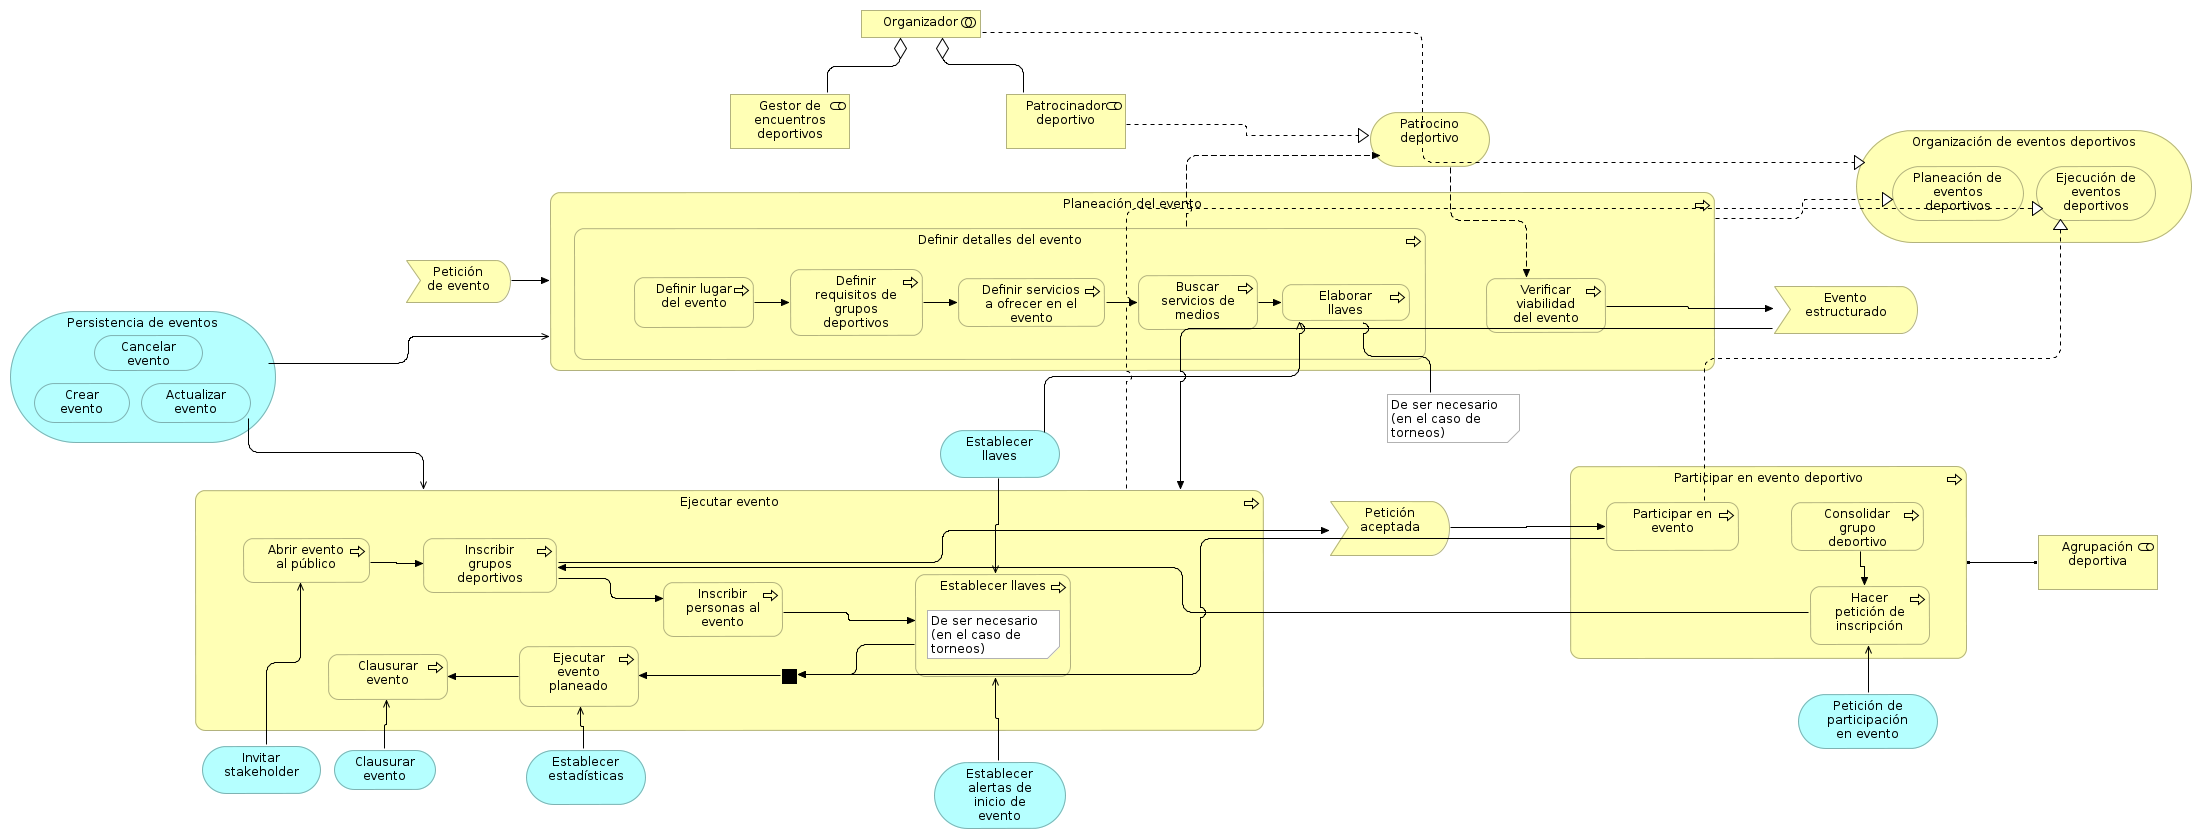
\includegraphics[width=11cm]{./imagenes/business_process/organizacioneventosdeportivos.png}
    \caption{Buscador deportivo}
    \label{fig:BF_BuscadorDeportivo}
    \textbf{Fuente:}  Autores
  \end{center}
\end{figure}

\begin{table}[!htb]
	\caption{Organización de Eventos Deportivos}
	\label{tab:BP_OrganizacionEventosDeportivos}
	\begin{center}
		\resizebox{11cm}{!}{
		\begin{tabular}{|p{7cm}|p{4cm}|}
			\hline
			Responsabilidades & Vistas relacionadas \\
			\hline \hline
			Administra el consumo y oferta de servicios deportivos a los interesados.
			\begin{itemize}
				\item \textbf{Entrenador deportivo (Rol):} 
				\item \textbf{Gestor de encuentros deportivos (Rol):} 
				\item \textbf{Agrupación deportiva (Rol):} 
				\item \textbf{Construcción de proyectos (Servicio de negocio):} 
				\item \textbf{Evaluación de proyectos (Servicio de negocio):} 
				\item \textbf{Patrocinio deportivo (Servicio de negocio):} 
				\item \textbf{Necesidad de patrocinio (Evento):} 
				\item \textbf{Petición de patrocinio (Evento):} 
				\item \textbf{Pedir patrocinio (Proceso de negocio):} 
				\item \textbf{Realizar proyecto a presentar (Proceso de negocio):} 
				\item \textbf{Enviar proyecto a patrocinadores (Proceso de negocio):} 
				\item \textbf{Calcular costo/beneficio de patrocinio (Proceso de negocio):} 
				\item \textbf{Evaluar financiamiento (Proceso de negocio):} 
				\item \textbf{Evaluar préstamo de servicio (Proceso de negocio):} 
				\item \textbf{Evaluar préstamo de producto (Proceso de negocio):} 
				\item \textbf{Patrocinar (Proceso de negocio):} 
				\item \textbf{Buscar servicio (Proceso de negocio):} 
				\item \textbf{Prestar servicio (Proceso de negocio):} 
				\item \textbf{Buscar material deportivo (Proceso de negocio):} 
				\item \textbf{Dar producto deportivo (Proceso de negocio):} 
				\item \textbf{Financiar evento deportivo (Proceso de negocio):} 
				\item \textbf{Financiar grupo deportivo (Proceso de negocio):} 
				\item \textbf{Pedir patrocinio (Servicio de aplicación):} 
				\item \textbf{Persistencia de servicios (Servicio de aplicación):}  datos de servicios
				\item \textbf{Actualizar servicio (Servicio de aplicación):} 
				\item \textbf{Crear servicio (Servicio de aplicación):} 
				\item \textbf{Consultar servicio (Servicio de aplicación):} 
				\item \textbf{Calcular rendimiento (Servicio de aplicación):} 
				\item \textbf{Modificar capacidad financiadora (Servicio de aplicación):} 
				\item \textbf{Gestión de patrocinios (Servicio de aplicación):} 
				\item \textbf{Persistencia de recursos materiales (Servicio de aplicación):} 
				\item \textbf{Actualizar recursos materiales (Servicio de aplicación):} 
				\item \textbf{Crear recursos materiales (Servicio de aplicación):} 
				\item \textbf{Consultar recursos materiales (Servicio de aplicación):} 
			\end{itemize} 
			&
			\begin{itemize}
				\item N/A
			\end{itemize} 
			\\
			\hline
		\end{tabular}
		} \\
		\textbf{Fuente}: Autores
	\end{center}
\end{table}

\subsubsection{Formación de Grupos Deportivos}

\begin{figure}[!htb]
  \begin{center}
    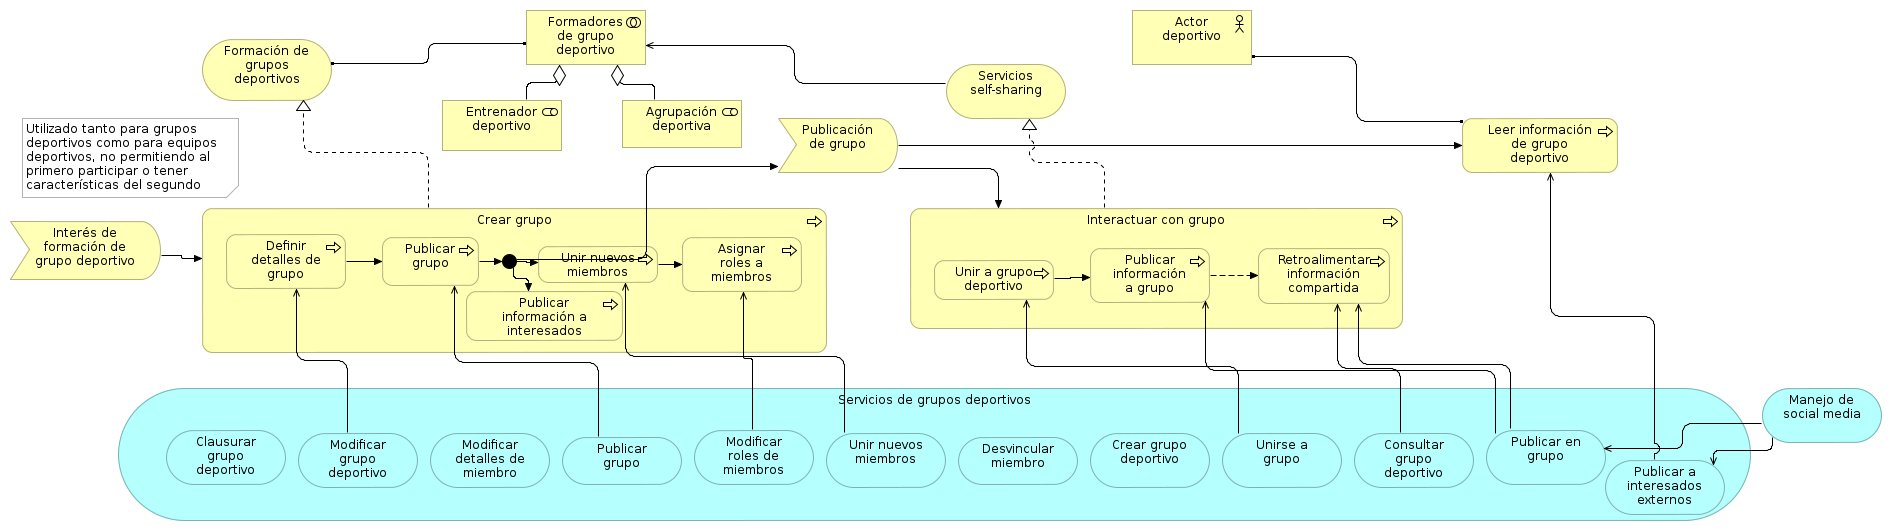
\includegraphics[width=11cm]{./imagenes/business_process/formaciongruposdeportivos.png}
    \caption{Buscador deportivo}
    \label{fig:BF_BuscadorDeportivo}
    \textbf{Fuente:}  Autores
  \end{center}
\end{figure}

\clearpage

\subsubsection{Estadísticas Deportivas}

\begin{figure}[!htb]
  \begin{center}
    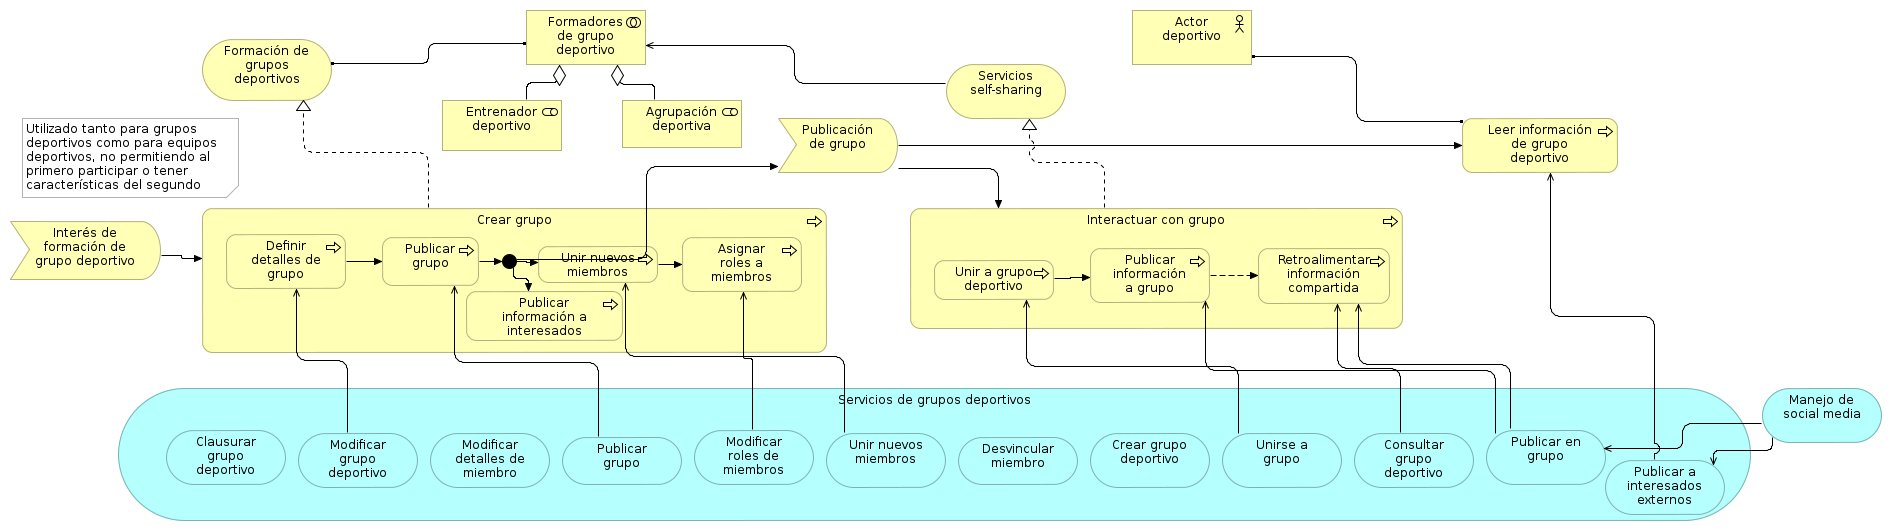
\includegraphics[width=11cm]{./imagenes/business_process/estadisticasdeportivas.png}
    \caption{Buscador deportivo}
    \label{fig:BF_BuscadorDeportivo}
    \textbf{Fuente:}  Autores
  \end{center}
\end{figure}

\subsubsection{Entrenamiento Deportivo}

\begin{figure}[!htb]
  \begin{center}
    \includegraphics[width=11cm]{./imagenes/business_process/entrenamientodeportivo.png}
    \caption{Buscador deportivo}
    \label{fig:BF_BuscadorDeportivo}
    \textbf{Fuente:}  Autores
  \end{center}
\end{figure}

\subsubsection{Buscador de consejos deportivos}

\begin{figure}[!htb]
  \begin{center}
    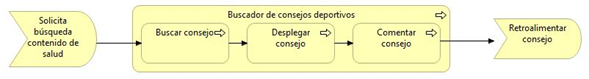
\includegraphics[width=11cm]{./imagenes/business_process/buscadorconsejosdeportivos.png}
    \caption{Buscador de consejos deportivos}
    \label{fig:BP_BuscadorConsejosDeportivos}
    \textbf{Fuente:}  Autores
  \end{center}
\end{figure}

\begin{table}[!htb]
	\caption{Descripción Buscador de consejos deportivos}
	\label{tab:BP_BuscadorConsejosDeportivos}
	\begin{center}
		\resizebox{11cm}{!}{
		\begin{tabular}{|p{7cm}|p{4cm}|}
			\hline
			Responsabilidades & Vistas relacionadas \\
			\hline \hline
			Proceso por el cual se hacen las búsquedas de consejos relacionados a un tema de interés.
			\begin{itemize}
				\item \textbf{Solicita búsqueda contenido de salud (Evento):} Evento por el cual un interesado genera la búsqueda de un contenido de salud.
				\item \textbf{Retroalimentar consejo (Evento):} Evento que se genera luego de que un consejo consultado es utilizado y se comenta su utilidad.
				\item \textbf{Buscar consejo (Proceso):} Proceso encargado de buscar un consejo en una base de conocimiento
				\item \textbf{Desplegar consejo (Proceso):} Proceso encargado de, a partir de un consejo seleccionado, desplegar la información relacionada a un consejo.
				\item \textbf{Comentar consejo (Proceso):} Proceso encargado de registrar el comentario generado por un usuario luego de utilizar un consejo consultado con el buscador de consejos deportivos.
			\end{itemize} 
			&
			\begin{itemize}
				\item N/A
			\end{itemize} 
			\\
			\hline
		\end{tabular}
		} \\
		\textbf{Fuente}: Autores
	\end{center}
\end{table}

\subsubsection{Buscador deportivo}

\begin{figure}[!htb]
  \begin{center}
    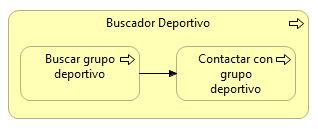
\includegraphics[width=11cm]{./imagenes/business_process/buscadordeportivo.png}
    \caption{Buscador deportivo}
    \label{fig:BP_BuscadorDeportivo}
    \textbf{Fuente:}  Autores
  \end{center}
\end{figure}

\begin{table}[!htb]
	\caption{Descripción Buscador deportivo}
	\label{tab:BP_BuscadorDeportivo}
	\begin{center}
		\resizebox{11cm}{!}{
		\begin{tabular}{|p{7cm}|p{4cm}|}
			\hline
			Responsabilidades & Vistas relacionadas \\
			\hline \hline
			Proceso que se encarga de buscar un grupo deportivo y facilitar su contacto.
			\begin{itemize}
				\item \textbf{Buscar grupo deportivo (Proceso):} Proceso que busca en la base de conocimientos los grupos deportivos que cumplan ciertos criterios de búsqueda 
				\item \textbf{Contactar con grupo deportivo (Proceso):} Proceso que facilita el contacto de grupos deportivos, exponiendo los datos de contacto suministrados por cada grupo y medios para la comunicación.

			\end{itemize} 
			&
			\begin{itemize}
				\item N/A
			\end{itemize} 
			\\
			\hline
		\end{tabular}
		} \\
		\textbf{Fuente}: Autores
	\end{center}
\end{table}

\subsubsection{Evaluador consejos de salud}

\begin{figure}[!htb]
  \begin{center}
    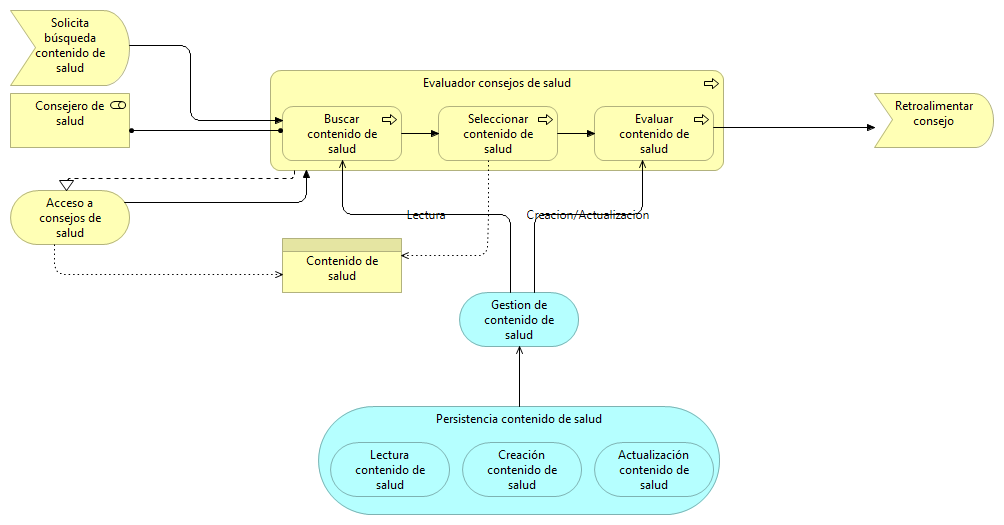
\includegraphics[width=11cm]{./imagenes/business_process/evaluadorconsejossalud.png}
    \caption{Evaluador consejos de salud}
    \label{fig:BP_EvaluadorConsejosSalud}
    \textbf{Fuente:}  Autores
  \end{center}
\end{figure}

\begin{table}[!htb]
	\caption{Descripción Evaluador consejos de salud}
	\label{tab:BP_EvaluadorConsejosSalud}
	\begin{center}
		\resizebox{11cm}{!}{
		\begin{tabular}{|p{7cm}|p{4cm}|}
			\hline
			Responsabilidades & Vistas relacionadas \\
			\hline \hline
			Proceso por el cual se puede buscar y evaluar un consejo de salud.
			\begin{itemize}
				\item \textbf{Solicita búsqueda contenido de salud (Evento):} Evento por el cual un interesado genera la búsqueda de un contenido de salud.
				\item \textbf{Retroalimentar consejo (Evento):} Evento que se genera luego de que un contenido consultado es utilizado y se comenta su utilidad.
				\item \textbf{Buscar contenido de salud (Proceso):} Proceso encargado de buscar un contenido de salud en una base de conocimiento.
				\item \textbf{Seleccionar contenido de salud (Proceso):} Proceso encargado de, a partir de un contenido seleccionado, desplegar la información relacionada a un contenido.
				\item \textbf{Evaluar contenido de salud (Proceso):} Proceso encargado de registrar el comentario generado por un usuario luego de utilizar un contenido consultado con el buscador de contenidos de salud.
			\end{itemize} 
			&
			\begin{itemize}
				\item N/A
			\end{itemize} 
			\\
			\hline
		\end{tabular}
		} \\
		\textbf{Fuente}: Autores
	\end{center}
\end{table}

\clearpage

\subsubsection{Generador de consejos deportivos}

\begin{figure}[!htb]
  \begin{center}
    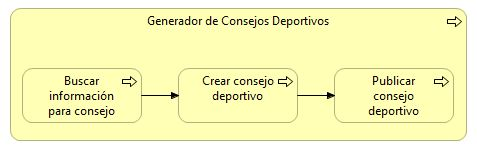
\includegraphics[width=11cm]{./imagenes/business_process/generadorconsejosdeportivos.png}
    \caption{Generador de consejos deportivos}
    \label{fig:BP_GeneradorConsejosDeportivos}
    \textbf{Fuente:}  Autores
  \end{center}
\end{figure}

\begin{table}[!htb]
	\caption{Generador de consejos deportivos}
	\label{tab:BP_GeneradorConsejosDeportivos}
	\begin{center}
		\resizebox{11cm}{!}{
		\begin{tabular}{|p{7cm}|p{4cm}|}
			\hline
			Responsabilidades & Vistas relacionadas \\
			\hline \hline
			Proceso por el cual se puede adicionar un nuevo consejo deportivo a la base de conocimientos. 
			\begin{itemize}
				\item \textbf{Buscar información para consejo (Proceso):} Proceso que permite la búsqueda de información relacionada a una temática deportiva.
				\item \textbf{Crear consejo deportivo (Proceso):} Proceso que permite la creación (cuerpo) de un consejo deportivo.
				\item \textbf{Publicar consejo deportivo (Proceso):} Proceso que facilita la publicación y registro de un consejo en una base de conocimientos.
			\end{itemize} 
			&
			\begin{itemize}
				\item N/A
			\end{itemize} 
			\\
			\hline
		\end{tabular}
		} \\
		\textbf{Fuente}: Autores
	\end{center}
\end{table}

\subsubsection{Generador de contenidos de salud}

\begin{figure}[!htb]
  \begin{center}
    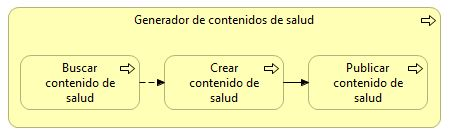
\includegraphics[width=11cm]{./imagenes/business_process/generadorcontenidossalud.png}
    \caption{Generador de contenidos de salud}
    \label{fig:BP_GeneradorContenidosSalud}
    \textbf{Fuente:}  Autores
  \end{center}
\end{figure}

\begin{table}[!htb]
	\caption{Generador de contenidos de salud}
	\label{tab:BP_GeneradorContenidosSalud}
	\begin{center}
		\resizebox{11cm}{!}{
		\begin{tabular}{|p{7cm}|p{4cm}|}
			\hline
			Responsabilidades & Vistas relacionadas \\
			\hline \hline
			Proceso por el cual se puede adicionar un nuevo contenido de salid a la base de conocimientos. 
			\begin{itemize}
				\item \textbf{Buscar contenido de salud (Proceso):} Proceso que permite la búsqueda de información relacionada a una temática de salud.
				\item \textbf{Crear contenido de salud (Proceso):} Proceso que permite la creación (cuerpo) de un consejo de salud.
				\item \textbf{Publicar contenido de salud (Proceso):} Proceso que facilita la publicación y registro de un contenido de salud en una base de conocimientos.
			\end{itemize} 
			&
			\begin{itemize}
				\item N/A
			\end{itemize} 
			\\
			\hline
		\end{tabular}
		} \\
		\textbf{Fuente}: Autores
	\end{center}
\end{table}

\subsection{Application Usage Viewpoints}

\subsubsection{Patrocinios Deportivos}

\begin{figure}[!htb]
  \begin{center}
    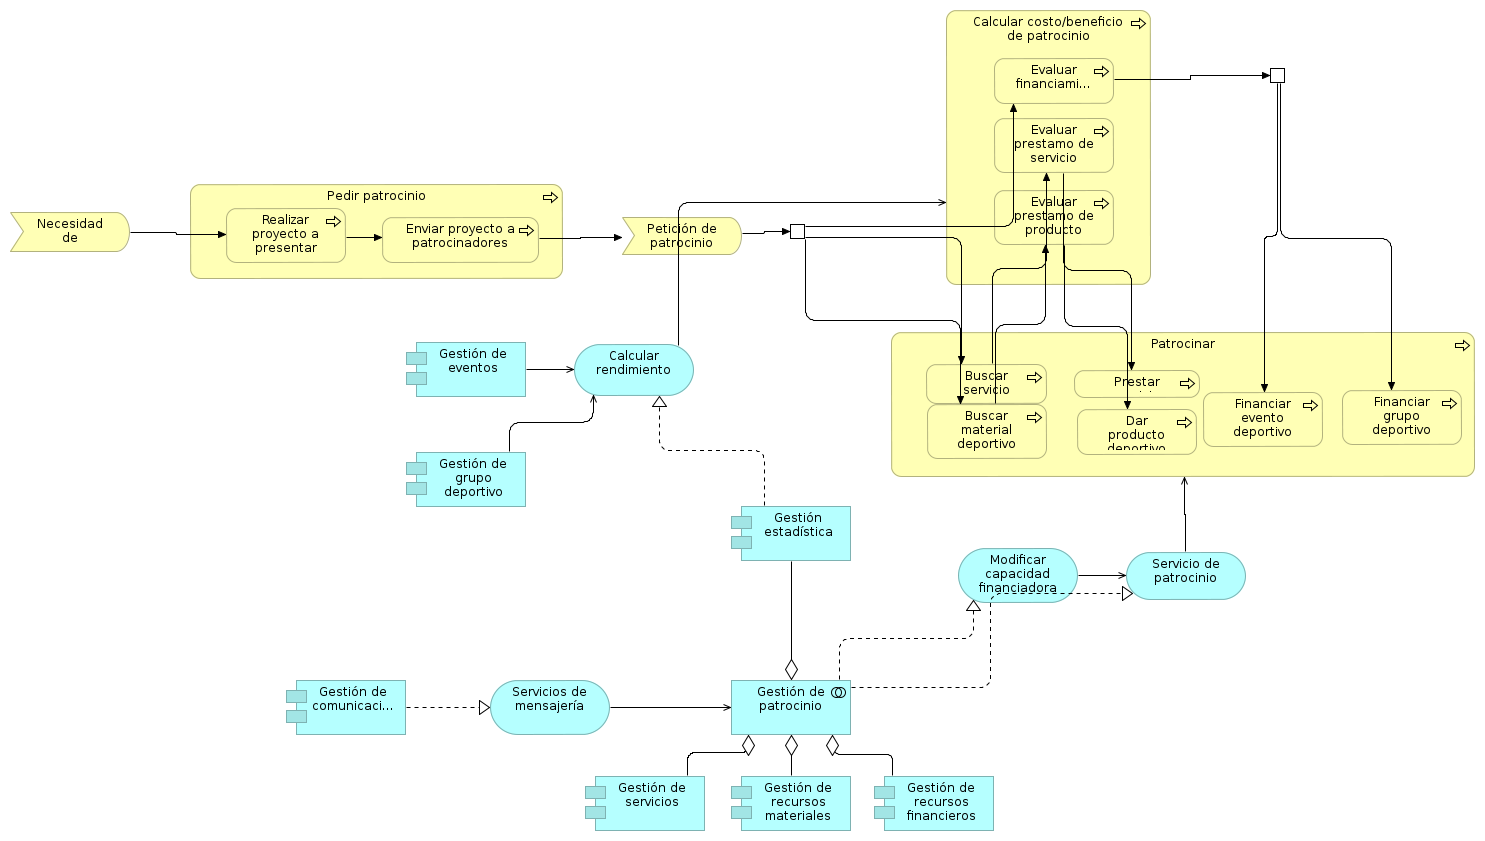
\includegraphics[width=11cm]{./imagenes/application_usage/patrociniosdeportivos.png}
    \caption{Buscador deportivo}
    \label{fig:BF_BuscadorDeportivo}
    \textbf{Fuente:}  Autores
  \end{center}
\end{figure}

\begin{table}[!htb]
	\caption{Patrocinios Deportivos}
	\label{tab:BP_PatrociniosDeportivos}
	\begin{center}
		\resizebox{11cm}{!}{
		\begin{tabular}{|p{7cm}|p{4cm}|}
			\hline
			Responsabilidades & Vistas relacionadas \\
			\hline \hline
			Administra el consumo y oferta de servicios deportivos a los interesados.
			\begin{itemize}
				\item \textbf{Necesidad de patrocinio (Evento):} Establece una necesidad de que un evento/actor deportivo necesite de un patrocinio deportivo
				\item \textbf{Petición de patrocinio (Evento):} Realiza la petición de patrocinio a un patrocinador deportivo
				\item \textbf{Pedir patrocinio (Proceso de negocio):} Proceso por el cual los actores deportivos interesados hacen una petición de patrocinio a los patrocinadores identificados en la red social
				\item \textbf{Realizar proyecto a presentar (Proceso de negocio):} Realiza la construcción del proyecto a presentar a los patrocinadores deportivos
				\item \textbf{Enviar proyecto a patrocinadores (Proceso de negocio):} Envía el proyecto a los patrocinadores deportivos que haya elegido el actor deportivo interesado
				\item \textbf{Calcular costo/beneficio de patrocinio (Proceso de negocio):} Realiza un cálculo de costo/beneficio para dar herramientas que le permitan al patrocinador evaluar si es viable o no un patrocinio
				\item \textbf{Evaluar financiamiento (Proceso de negocio):} Evalúa el financiamiento del proyecto presentado por un actor deportivo
				\item \textbf{Evaluar préstamo de servicio (Proceso de negocio):} Evalúa el préstamo de un servicio como patrocinio al proyecto de un actor deportivo
				\item \textbf{Evaluar préstamo de producto (Proceso de negocio):} Evalúa el préstamo de materiales que puedan ser prestados/regalados como patrocinio a un proyecto presentado por un actor deportivo
				\item \textbf{Patrocinar (Proceso de negocio):} Proceso de patrocinio de un proyecto presentado por un actor deportivo
				\item \textbf{Buscar servicio (Proceso de negocio):} Busca los servicios prestados que puedan ayudar al proyecto a patrocinar de algún modo
				\item \textbf{Prestar servicio (Proceso de negocio):} Presta los servicios prestados que puedan ayudar al proyecto a patrocinar de algún modo
				\item \textbf{Buscar material deportivo (Proceso de negocio):} Busca los productos prestados que puedan ayudar al proyecto a patrocinar de algún modo
				\item \textbf{Dar producto deportivo (Proceso de negocio):} Da los productos deportivos que puedan ayudar al proyecto a patrocinar de algún modo
				\item \textbf{Financiar evento deportivo (Proceso de negocio):} Financia un evento deportivo
				\item \textbf{Financiar grupo deportivo (Proceso de negocio):} Financia las actividades de una agrupación deportiva
				\item \textbf{Pedir patrocinio (Servicio de aplicación):} Servicio desde el cual un actor deportivo pide un patrocinio a un patrocinador
				\item \textbf{Persistencia de servicios (Servicio de aplicación):} Servicio para el manejo de datos de servicios
				\item \textbf{Actualizar servicio (Servicio de aplicación):} Actualiza un servicio ofrecido
				\item \textbf{Crear servicio (Servicio de aplicación):} Permite la creación de un servicio
				\item \textbf{Consultar servicio (Servicio de aplicación):} Permite la consulta de la información de un servicio
				\item \textbf{Calcular rendimiento (Servicio de aplicación):} Calcula las ganancias/perdidas que se tendrán al tomar el rol de patrocinador de un evento/actor deportivo
				\item \textbf{Modificar capacidad financiadora (Servicio de aplicación):} Manejo de la capacidad de financiamiento (o préstamo de servicio o producto) al actor deportivo para la realización del proyecto
				\item \textbf{Gestión de patrocinios (Servicio de aplicación):} Utiliza los servicios que ponen a disposición patrocinadores para patrocinar eventos deportivo o actores deportivos
				\item \textbf{Persistencia de recursos materiales (Servicio de aplicación):} Servicio para el manejo de los datos referentes a los recursos materiales de un actor comercial
				\item \textbf{Actualizar recursos materiales (Servicio de aplicación):} Actualiza loa información de los recursos materiales
				\item \textbf{Crear recursos materiales (Servicio de aplicación):} Este servicio ofrece la creación de recursos materiales
				\item \textbf{Consultar recursos materiales (Servicio de aplicación):} Deja consultar la información de recursos materiales
				\item \textbf{Gestión de eventos (Componente de aplicación):} Realiza todas las funcionalidades ofrecidas en los servicios de eventos (creación, modificación y consulta, así como también funcionalidades estadísticas por medio del componente "Gestión estadística")
				\item \textbf{Gestión de grupo deportivo (Componente de aplicación):} Módulo para la gestión de grupos deportivos
				\item \textbf{Gestión estadística (Componente de aplicación):} Componente usado por otros para la producción de información estadística en cuanto a los criterios establecidos para cada actor deportivo, para cada evento deportivo y para cada servicio deportivo prestado
				\item \textbf{Gestión de comunicación (Componente de aplicación):} Sirve como componente administrador de las funciones chat del SNS
				\item \textbf{Gestión de recursos materiales (Componente de aplicación):} Gestión de recursos materiales para patrocinio de un patrocinador
				\item \textbf{Gestión de servicios (Componente de aplicación):} Colabora (por la parte del prestador de servicios) en la producción de la relación compra-venta entre actores-usuarios de la red social deportiva
				\item \textbf{Gestión de recursos financieros (Componente de aplicación):} Gestión de recursos financieros para patrocinio de un patrocinador
				\item \textbf{Servicio de mensajería (Servicio de aplicación):} Servicio de comunicación instantánea entre el patrocinador y el actor deportivo que presentó el proyecto
			\end{itemize} 
			&
			\begin{itemize}
				\item Application usage (Patrocinio deportivo)
				\item Application usage (Patrocinio deportivo)
				\item Application usage (Patrocinio deportivo)
				\item Application usage (Patrocinio deportivo)
				\item Application usage (Patrocinio deportivo)
				\item Application usage (Patrocinio deportivo)
				\item Application usage (Patrocinio deportivo)
				\item Application usage (Patrocinio deportivo)
				\item Application usage (Patrocinio deportivo)
				\item Application usage (Patrocinio deportivo)
				\item Application usage (Patrocinio deportivo)
				\item Application usage (Patrocinio deportivo)
				\item Application usage (Patrocinio deportivo)
				\item Application usage (Patrocinio deportivo)
				\item Application usage (Patrocinio deportivo)
				\item Application usage (Patrocinio deportivo)
				\item Application usage (Patrocinio deportivo)
				\item Application usage (Patrocinio deportivo)
				\item Application usage (Patrocinio deportivo)
				\item Application usage (Patrocinio deportivo)
				\item Application usage (Patrocinio deportivo)
				\item Application usage (Patrocinio deportivo)
				\item Application usage (Patrocinio deportivo)
				\item Business process (Organización de eventos deportivos) ,Application usage (Organización de eventos deportivos, Patrocinio deportivo)
				\item Application usage (Patrocinio deportivo)
				\item Application usage (Patrocinio deportivo)
				\item Application usage (Patrocinio deportivo)
				\item Application usage (Patrocinio deportivo
				\item Application usage (Patrocinio deportivo)
				\item General layered, Application usage (Estadísticas deportivas, Organización eventos deportivos)
				\item Application usage (Formación de grupos deportivos, Entrenamiento deportivo)
				\item General layered, Application usage (Entrenamiento deportivo, Estadísticas deportivas, Organización de eventos deportivos)
				\item Application usage (Entrenamiento deportivo, Formación de grupos deportivos)
				\item N/A
				\item General layered, Application usage (Entrenamiento deportivo, Estadisticas deportivas)
				\item N/A
				\item N/A
			\end{itemize} 
			\\
			\hline
		\end{tabular}
		} \\
		\textbf{Fuente}: Autores
	\end{center}
\end{table}

\subsubsection{Organización de Eventos Deportivos}

\begin{figure}[!htb]
  \begin{center}
    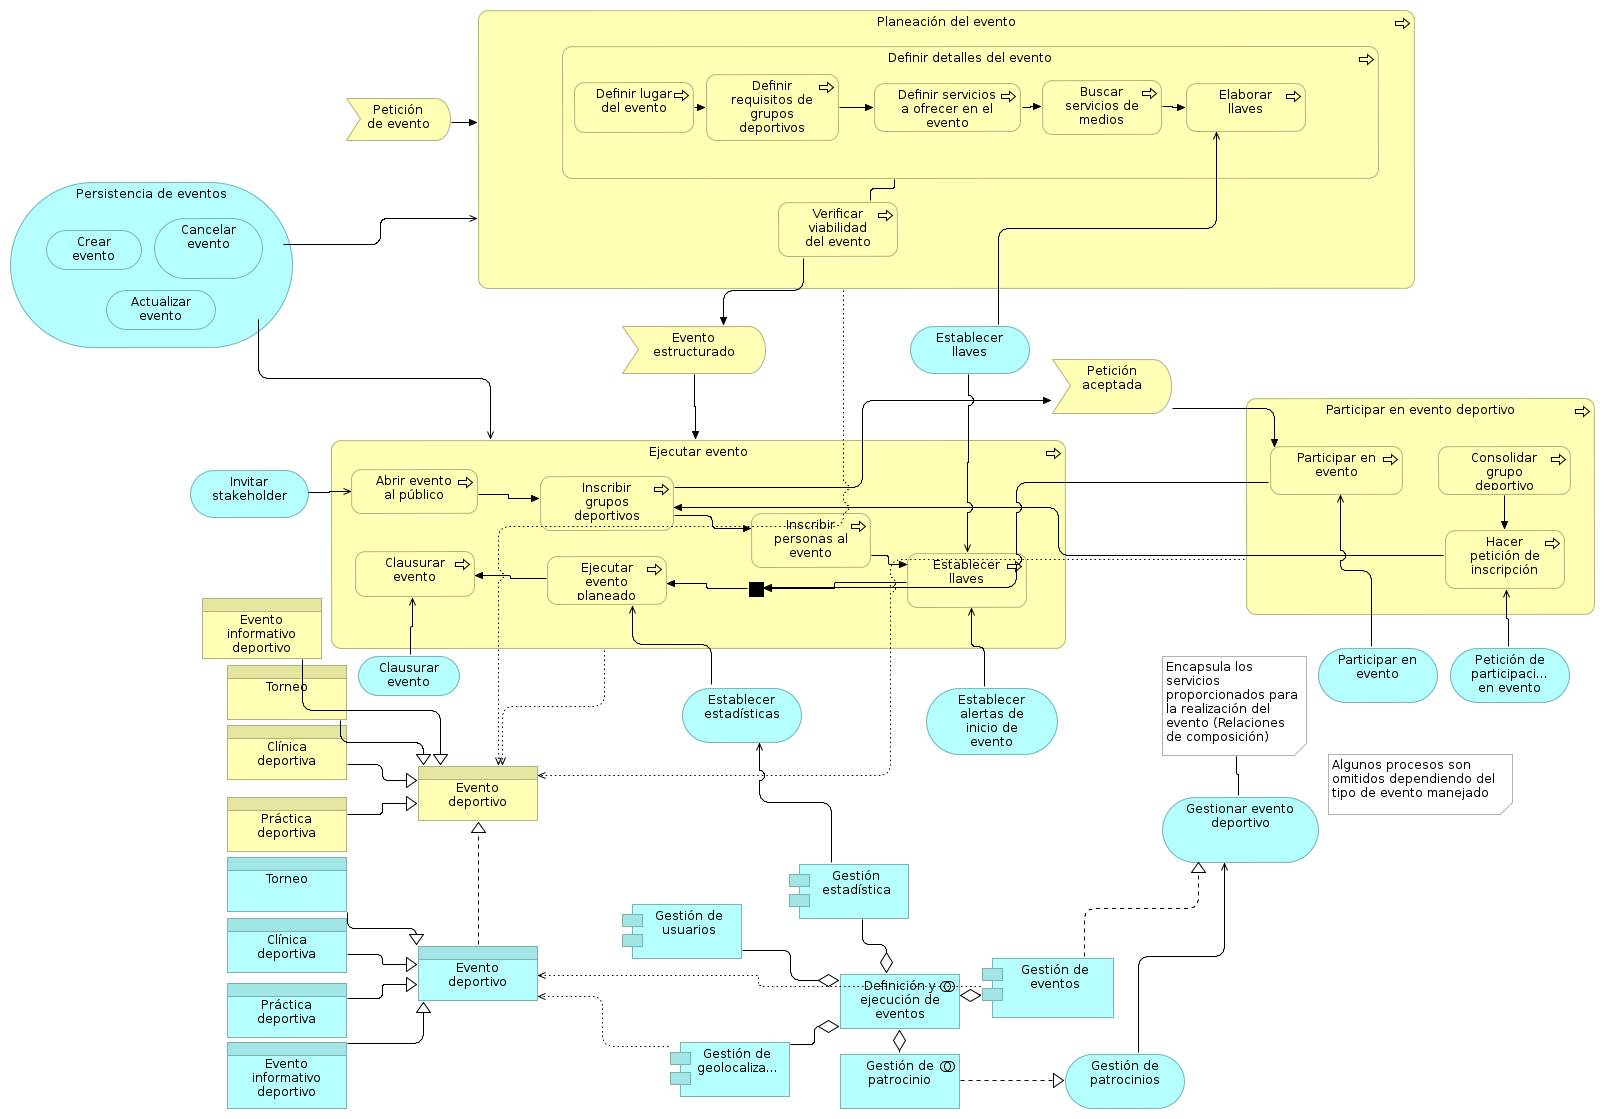
\includegraphics[width=11cm]{./imagenes/application_usage/organizacioneventosdeportivos.png}
    \caption{Buscador deportivo}
    \label{fig:BF_BuscadorDeportivo}
    \textbf{Fuente:}  Autores
  \end{center}
\end{figure}

\subsubsection{Formación de Grupos Deportivos}

\begin{figure}[!htb]
  \begin{center}
    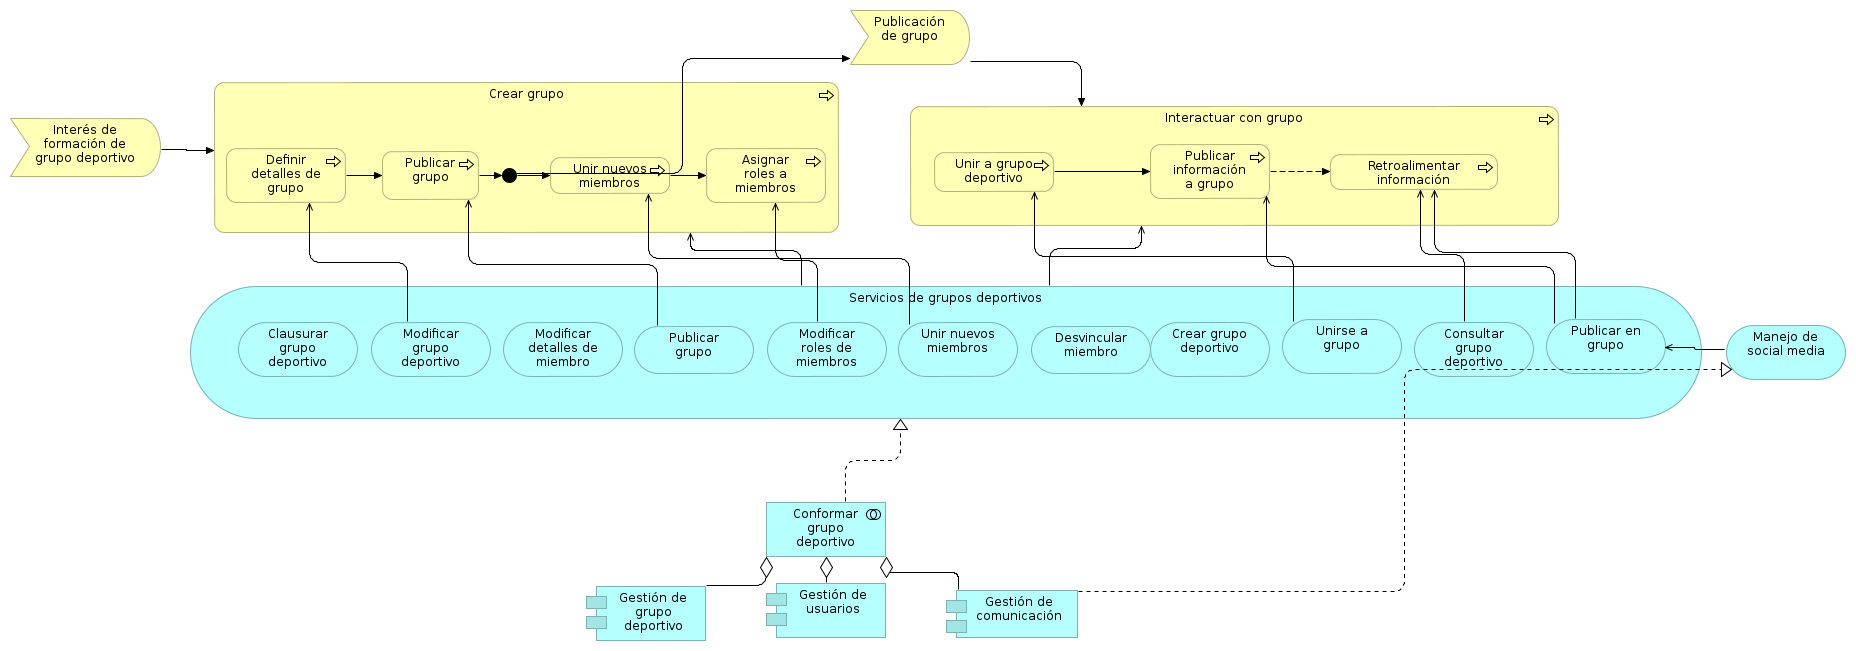
\includegraphics[width=11cm]{./imagenes/application_usage/formaciongruposdeportivos.png}
    \caption{Buscador deportivo}
    \label{fig:BF_BuscadorDeportivo}
    \textbf{Fuente:}  Autores
  \end{center}
\end{figure}

\subsubsection{Estadísticas Deportivas}

\begin{figure}[!htb]
  \begin{center}
    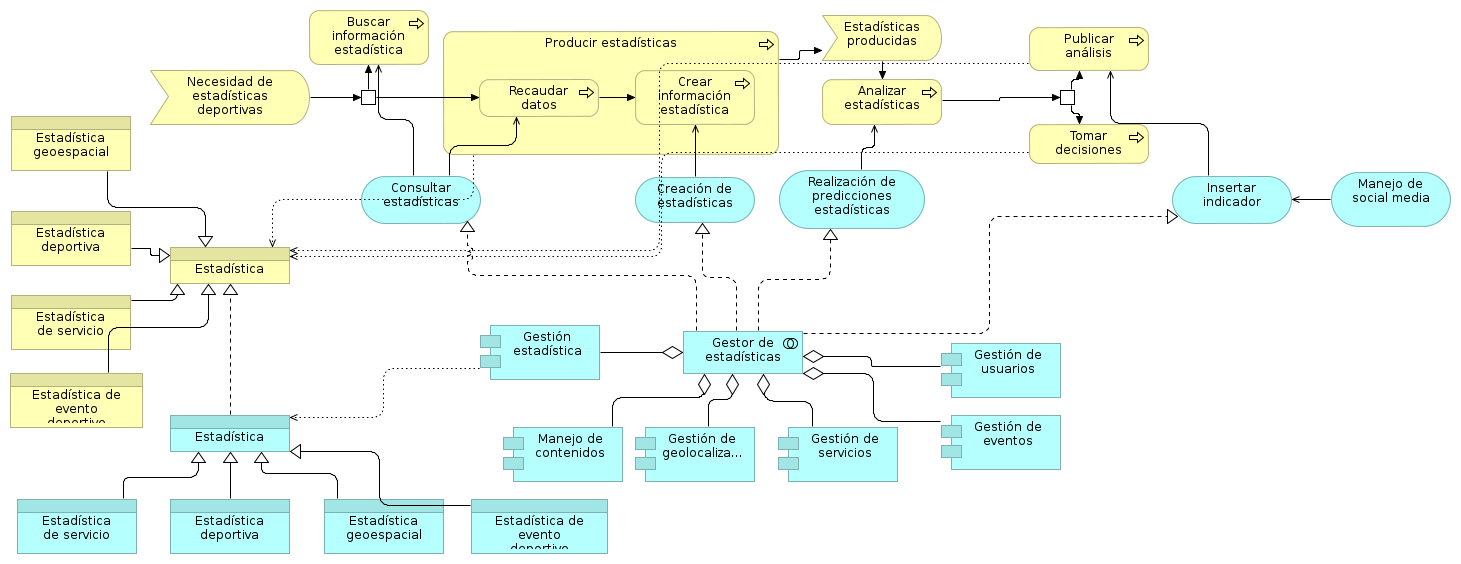
\includegraphics[width=11cm]{./imagenes/application_usage/estadisticasdeportivas.png}
    \caption{Buscador deportivo}
    \label{fig:BF_BuscadorDeportivo}
    \textbf{Fuente:}  Autores
  \end{center}
\end{figure}

\subsubsection{Entrenamiento Deportivo}

\begin{figure}[!htb]
  \begin{center}
    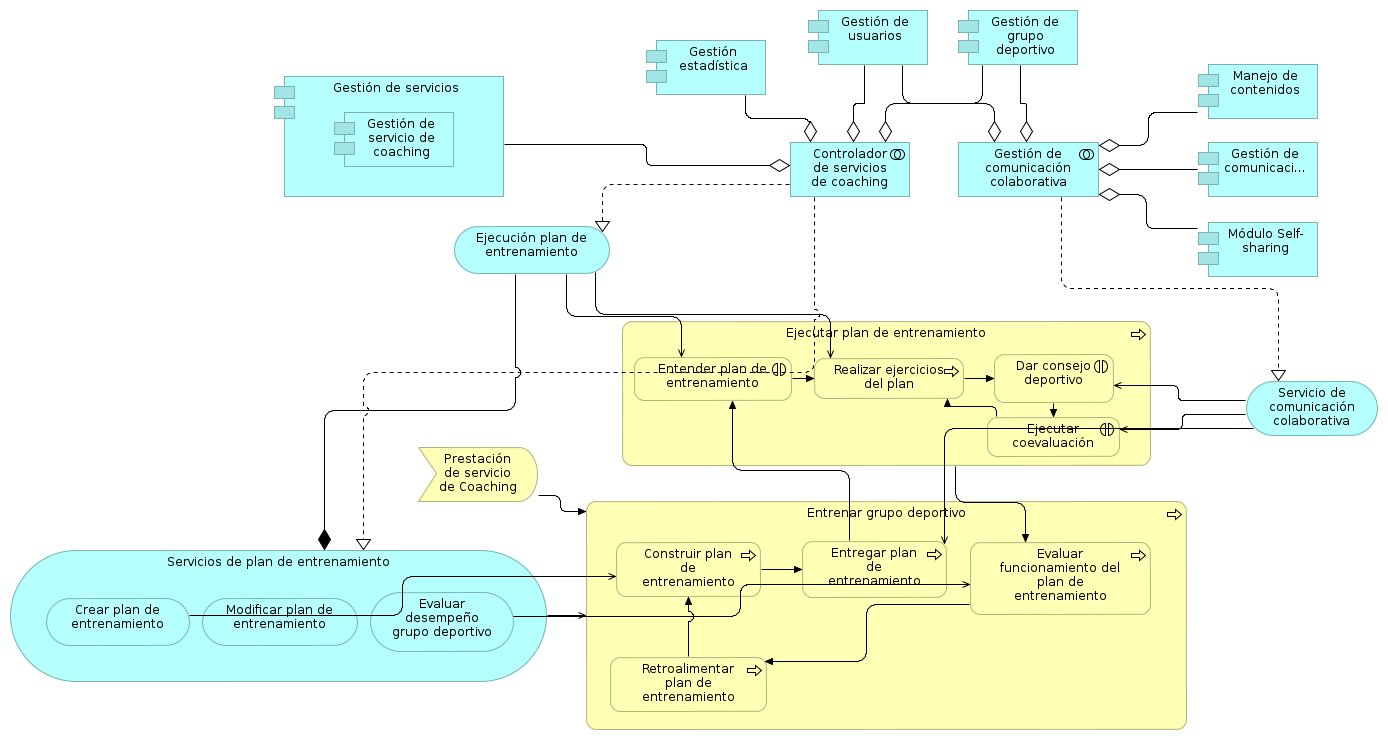
\includegraphics[width=11cm]{./imagenes/application_usage/entrenamientodeportivo.png}
    \caption{Buscador deportivo}
    \label{fig:BF_BuscadorDeportivo}
    \textbf{Fuente:}  Autores
  \end{center}
\end{figure}

\subsubsection{Buscador de consejos deportivos}

\begin{figure}[!htb]
  \begin{center}
    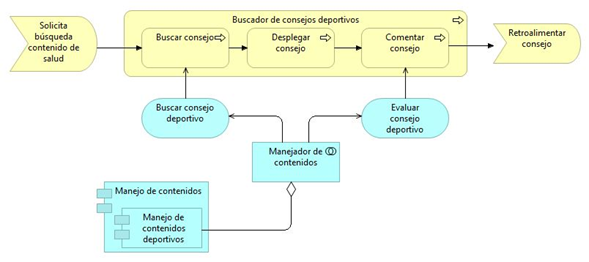
\includegraphics[width=11cm]{./imagenes/application_usage/buscadorconsejosdeportivos.png}
    \caption{Buscador de consejos deportivos}
    \label{fig:BP_BuscadorConsejosDeportivos}
    \textbf{Fuente:}  Autores
  \end{center}
\end{figure}

\begin{table}[!htb]
	\caption{Buscador de consejos deportivos}
	\label{tab:AU_BuscadorConsejosDeportivos}
	\begin{center}
		\resizebox{11cm}{!}{
		\begin{tabular}{|p{7cm}|p{4cm}|}
			\hline
			Responsabilidades & Vistas relacionadas \\
			\hline \hline
			\begin{itemize}
				\item \textbf{Buscar consejo deportivo (Servicio):} Servicio encargado de, a partir de los parámetros de búsqueda suministrados por un usuario, buscar en la base de conocimientos consejos deportivos.
				\item \textbf{Evaluar consejo deportivo (Servicio):} Servicio que registra la información de retroalimentación de un consejo deportivo existente en la base de conocimientos de la Aplicación
				\item \textbf{Manejador de contenidos (Colaboración):} Colaboración encargada de orquestar las acciones necesarias para el acceso, creación o modificación de contenidos de la Aplicación.
				\item \textbf{Manejo de contenidos deportivos (Componente):} Componente encargado de controlar el acceso a la base de conocimientos de contenidos deportivos de la Aplicación.
			\end{itemize} 
			&
			\begin{itemize}
				\item N/A
			\end{itemize} 
			\\
			\hline
		\end{tabular}
		} \\
		\textbf{Fuente}: Autores
	\end{center}
\end{table}

\clearpage

\subsubsection{Buscador deportivo}

\begin{figure}[!htb]
  \begin{center}
    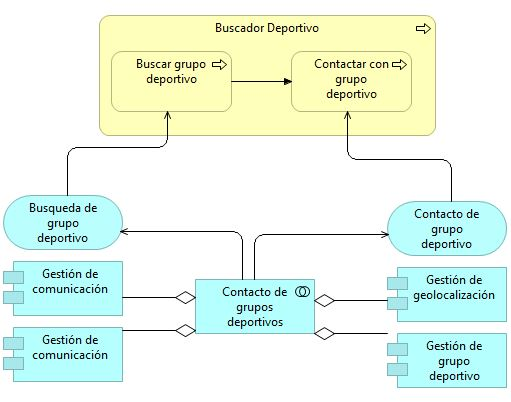
\includegraphics[width=11cm]{./imagenes/application_usage/buscadordeportivo.png}
    \caption{Buscador deportivo}
    \label{fig:BP_BuscadorDeportivo}
    \textbf{Fuente:}  Autores
  \end{center}
\end{figure}

\begin{table}[!htb]
	\caption{Buscador deportivo}
	\label{tab:AU_BuscadorDeportivo}
	\begin{center}
		\resizebox{11cm}{!}{
		\begin{tabular}{|p{7cm}|p{4cm}|}
			\hline
			Responsabilidades & Vistas relacionadas \\
			\hline \hline
			\begin{itemize}
				\item \textbf{búsqueda de grupo deportivo (Servicio):} Servicio encargado de buscar los grupos deportivos que cumplan con los criterios de búsqueda especificados por el usuario.
				\item \textbf{Contacto de grupo deportivo (Servicio):} Servicio que gestiona el contacto de grupos deportivos, exponiendo los datos de contacto suministrados por cada grupo y medios para la comunicación.
				\item \textbf{Contacto de grupos deportivos (Colaboración):} Colaboración que orquesta las acciones necesarias para la gestión y contacto de grupos deportivos al interior de la Aplicación.
				\item \textbf{gestión de comunicación (Componente):} Componente encargado de gestionar el paso de información entre dos o más grupos deportivos al interior de la Aplicación.
				\item \textbf{gestión de geo-localización (Componente):} Componente encargado de obtener y suministrar la ubicación de cada usuario al SNS.
				\item \textbf{gestión de grupo deportivo (Componente):} Componente encargado de administrar los grupos deportivos de la Aplicación (Crear, modificar, actualizar, eliminar), así como también debe gestionar el acceso a ésta información.
			\end{itemize} 
			&
			\begin{itemize}
				\item N/A
			\end{itemize} 
			\\
			\hline
		\end{tabular}
		} \\
		\textbf{Fuente}: Autores
	\end{center}
\end{table}

\subsubsection{Evaluador consejos de salud}

\begin{figure}[!htb]
  \begin{center}
    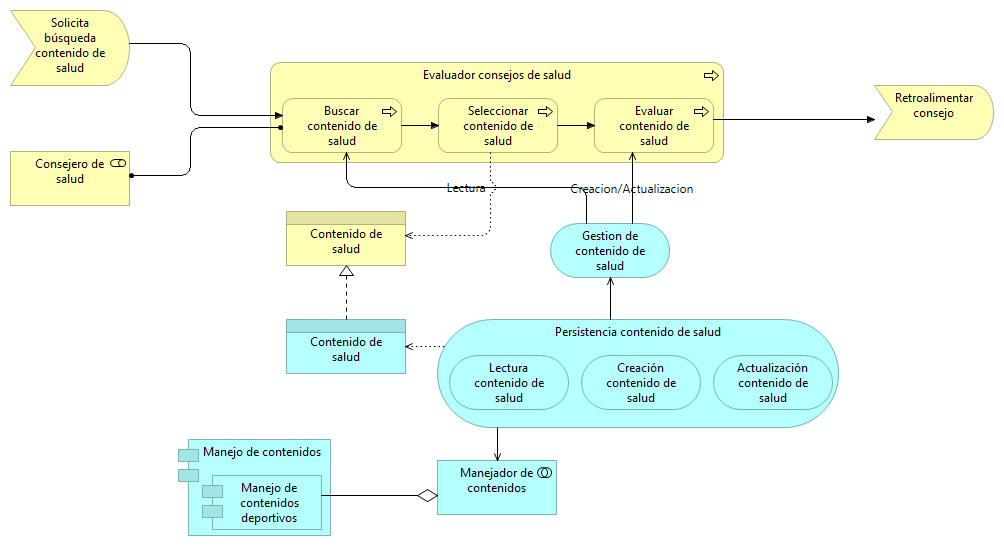
\includegraphics[width=11cm]{./imagenes/application_usage/evaluadorconsejossalud.png}
    \caption{Evaluador consejos de salud}
    \label{fig:BP_EvaluadorConsejosSalud}
    \textbf{Fuente:}  Autores
  \end{center}
\end{figure}

\begin{table}[!htb]
	\caption{Evaluador consejos de salud}
	\label{tab:AU_EvaluadorConsejosSalud}
	\begin{center}
		\resizebox{11cm}{!}{
		\begin{tabular}{|p{7cm}|p{4cm}|}
			\hline
			Responsabilidades & Vistas relacionadas \\
			\hline \hline
			\begin{itemize}
				\item \textbf{Buscar contenido de salud (Servicio):} Servicio encargado de, a partir de los parámetros de búsqueda suministrados por un usuario, buscar en la base de conocimientos contenidos de salud.
				\item \textbf{Evaluar contenido de salud (Servicio):} Servicio que registra la información de retroalimentación de un contenido de salud existente en la base de conocimientos de la Aplicación
				\item \textbf{Manejador de contenidos (Colaboración):} Colaboración encargada de orquestar las acciones necesarias para el acceso, creación o modificación de contenidos de la Aplicación.
				\item \textbf{Manejo de contenidos de salud (Componente):} Componente encargado de controlar el acceso a la base de conocimientos de contenidos de salud de la Aplicación.
			\end{itemize} 
			&
			\begin{itemize}
				\item N/A
			\end{itemize} 
			\\
			\hline
		\end{tabular}
		} \\
		\textbf{Fuente}: Autores
	\end{center}
\end{table}

\subsubsection{Generador de consejos deportivos}

\begin{figure}[!htb]
  \begin{center}
    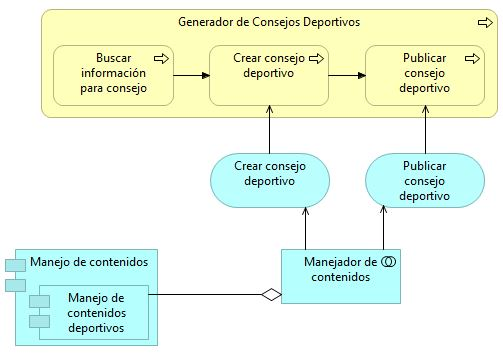
\includegraphics[width=11cm]{./imagenes/application_usage/generadorconsejosdeportivos.png}
    \caption{Generador de consejos deportivos}
    \label{fig:BP_GeneradorConsejosDeportivos}
    \textbf{Fuente:}  Autores
  \end{center}
\end{figure}

\begin{table}[!htb]
	\caption{Generador de consejos deportivos}
	\label{tab:AU_GeneradorConsejosDeportivos}
	\begin{center}
		\resizebox{11cm}{!}{
		\begin{tabular}{|p{7cm}|p{4cm}|}
			\hline
			Responsabilidades & Vistas relacionadas \\
			\hline \hline
			\begin{itemize}
				\item \textbf{Crear consejo deportivo (Servicio):} Servicio encargado de registrar un consejo deportivo relacionado a una temática especifica en la base de conocimientos.
				\item \textbf{Publicar consejo deportivo (Servicio):} Servicio encargado de hacer visibles los consejos deportivos reción creados (Después de una revisión?).
				\item \textbf{Manejador de contenidos (Colaboración):} Colaboración encargada de orquestar las acciones necesarias para el acceso, creación o modificación de contenidos de la Aplicación.
				\item \textbf{Manejo de contenidos deportivos (Componente):} Componente encargado de controlar el acceso a la base de conocimientos de contenidos deportivos de la Aplicación.
			\end{itemize} 
			&
			\begin{itemize}
				\item N/A
			\end{itemize} 
			\\
			\hline
		\end{tabular}
		} \\
		\textbf{Fuente}: Autores
	\end{center}
\end{table}

\subsubsection{Generador de contenidos de salud}

\begin{figure}[!htb]
  \begin{center}
    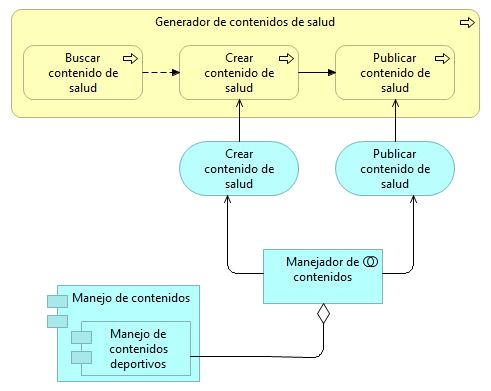
\includegraphics[width=11cm]{./imagenes/application_usage/generadorcontenidossalud.png}
    \caption{Generador de contenidos de salud}
    \label{fig:BP_GeneradorContenidosSalud}
    \textbf{Fuente:}  Autores
  \end{center}
\end{figure}

\begin{table}[!htb]
	\caption{Generador de contenidos de salud}
	\label{tab:AU_GeneradorContenidosSalud}
	\begin{center}
		\resizebox{11cm}{!}{
		\begin{tabular}{|p{7cm}|p{4cm}|}
			\hline
			Responsabilidades & Vistas relacionadas \\
			\hline \hline
			\begin{itemize}
				\item \textbf{Crear contenido de salud (Servicio):} Servicio encargado de registrar un contenido de salud relacionado a una temática especifica en la base de conocimientos.
				\item \textbf{Publicar contenido de salud (Servicio):} Servicio encargado de hacer visibles los contenidos de salud reción creados (Después de una revisión?).
				\item \textbf{Manejador de contenidos (Colaboración):} Colaboración encargada de orquestar las acciones necesarias para el acceso, creación o modificación de contenidos de la Aplicación.
				\item \textbf{Manejo de contenidos de salud (Componente):} Componente encargado de controlar el acceso a la base de conocimientos de contenidos de salud de la Aplicación.
			\end{itemize} 
			&
			\begin{itemize}
				\item N/A
			\end{itemize} 
			\\
			\hline
		\end{tabular}
		} \\
		\textbf{Fuente}: Autores
	\end{center}
\end{table}

\subsection{Product Viewpoint}

\subsubsection{Product}

\begin{figure}[!htb]
  \begin{center}
    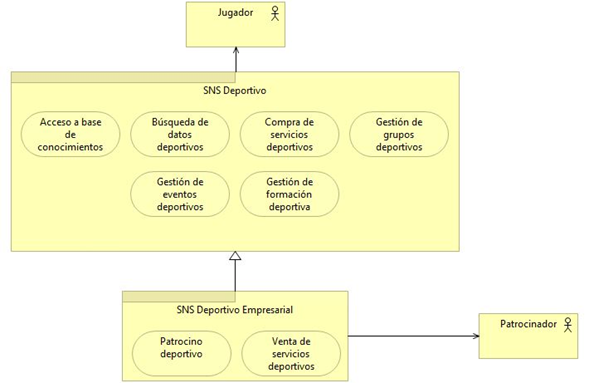
\includegraphics[width=11cm]{./imagenes/Product.png}
    \caption{Producto}
    \label{fig:Product}
    \textbf{Fuente:}  Autores
  \end{center}
\end{figure}

\clearpage

\begin{table}[!htb]
	\caption{Producto1}
	\label{tab:Product}
	\begin{center}
		\resizebox{11cm}{!}{
		\begin{tabular}{|p{7cm}|p{4cm}|}
			\hline
			Responsabilidades & Vistas relacionadas \\
			\hline \hline
			\begin{itemize}
				\item \textbf{Patrocinador (Actor):}
				\item \textbf{Jugador (Actor):}
				\item \textbf{SNS Deportivo (Producto):}
				\item \textbf{SNS Deportivo Empresarial (Producto):}
				\item \textbf{Acceso a base de conocimientos (Servicio):} Servicio que le permite al usuario acceder a las búsquedas, creación y evaluación de los contenidos almacenados en la base de conocimientos (Contenidos deportivos/de salud)
				\item \textbf{búsqueda de datos deportivos (Servicio):} Servicio que le permite al usuario acceder a los datos estadísticos de los diferentes deportes soportados por la Aplicación.
				\item \textbf{Compra de servicios deportivos (Servicio):} Servicio que le permite al usuario acceder al catálogo de servicios ofertados por los prestadores de servicios, pudiendo contactar, comprar y evaluar el servicio prestado por los mismos.
				\item \textbf{gestión de servicios deportivos (Servicio):} Servicio que le permite al usuario gestionar (Revisar, cancelar, renovar) los servicios deportivos/de salud adquiridos a través de la Aplicación.
				\item \textbf{gestión de eventos deportivos (Servicio):} Servicio que le permite al usuario gestionar (Crear, actualizar, modificar, eliminar, confirmar) los eventos deportivos, propios y ajenos, que se registran en la Aplicación.
				\item \textbf{gestión de formación deportiva (Servicio):} Servicio que le permite al usuario llevar un seguimiento de su formación y avance en la práctica de algún deporte registrado en la Aplicación.
				\item \textbf{Patrocinio deportivo (Servicio):} servicio que le permite al usuario empresarial administrar (Registrar, solicitar, ofrecer, crear, modificar, actualizar, eliminar) un patrocinio.
				\item \textbf{Venta de servicios deportivos (Servicio):} servicio que le permite al usuario empresarial administrar (Registrar, ofrecer, crear, modificar, actualizar, eliminar) productos o servicios para ofrecer en la Aplicación.
			\end{itemize} 
			&
			\begin{itemize}
				\item N/A
			\end{itemize} 
			\\
			\hline
		\end{tabular}
		} \\
		\textbf{Fuente}: Autores
	\end{center}
\end{table}